

\newpage


\section{Relating $\mfdec$ to Existing Complexities in the Hybrid Setting}

\subsection{Supporting lemmas}



\begin{lemma}\label{lem: triangular discri}
   Let $g: \Phi\to [0,G]$. For $\nu, \rho\in\Delta(\Phi)$, we have  
   \begin{align*}
       \E_{\phi\sim \rho}[g(\phi)] \leq 3\E_{\phi\sim \nu}[g(\phi)] + 2G\cdot D_{\textup{H}}^2(\nu, \rho),   
   \end{align*}
   where $D_{\textup{H}}^2$ is the Hellinger distance. 
\end{lemma}
\begin{proof}
    \begin{align*}
        \left|\E_{\phi\sim \rho}[g(\phi)] - \E_{\phi\sim \nu}[g(\phi)]\right| 
        &= \left|\sum_\phi (\rho(\phi) - \nu(\phi)) g(\phi)\right| \\
        &\leq \sqrt{\sum_\phi (\rho(\phi) + \nu(\phi)) g(\phi)^2 } \sqrt{\sum_\phi \frac{(\rho(\phi) - \nu(\phi))^2}{\rho(\phi) + \nu(\phi)}} \\
        &\leq \frac{1}{2} \E_{\phi\sim \rho}[g(\phi)] + \frac{1}{2} \E_{\phi\sim \nu}[g(\phi)] + \frac{G}{2} D_\Delta(\nu, \rho),    \numberthis \label{eq: triangle inequ}
    \end{align*}
    where 
    \begin{align*}
        D_\Delta(\nu, \rho) = \sum_\phi \frac{(\rho(\phi) - \nu(\phi))^2}{\rho(\phi) + \nu(\phi)}
    \end{align*}
    is the triangular discrimination. We can further bound it as 
    \begin{align*}
        D_\Delta(\nu, \rho) = \sum_\phi \frac{(\rho(\phi) - \nu(\phi))^2}{\rho(\phi) + \nu(\phi)} = \sum_\phi  \frac{(\sqrt{\rho(\phi)} - \sqrt{\nu(\phi)})^2(\sqrt{\rho(\phi)} +  \sqrt{\nu(\phi)})^2}{\rho(\phi) + \nu(\phi)} \leq 2D_{\textup{H}}^2(\nu,\rho).  
    \end{align*}
    Using this in \pref{eq: triangle inequ} and rearranging gives the desired inequality. 
\end{proof}

\begin{lemma}\label{lem: connecting two digdec hybrid}
    Suppose that $(\calM,\Phi)$ satisfy \pref{assum: avg err} with estimation function $\ellest_h(\phi; o_h)_j = f_\phi(s_h,a_h; \bm{e}_j) - \varphi(s_h,a_h)^\top \bm{e}_j - f_\phi(s_{h+1}; \bm{e}_j)$. Furthermore, assume that $(\calM, \Phi)$ is Bellman complete (\pref{def: adv bc}). Then \pref{assum: squared est err} holds with $\err_h(\phi', \phi; o_h) = \sum_{j=1}^d (f_{\phi'}(s_h,a_h; \bm{e}_j) - \varphi(s_h,a_h)^\top \bm{e}_j - f_{\phi}(s_{h+1}; \bm{e}_j))^2$ and 
    \begin{align*} 
        \mfdec_\eta^{\Phi, \tilD_{\sbe}} \leq \mfdec_\eta^{\Phi, \tilD_{\bi}}. 
    \end{align*}
\end{lemma}
\begin{proof}
   The proof is similar to that in the stochastic setting (\pref{lem: connecting two digdec}). 
\end{proof}

\begin{lemma}\label{lem: reward same}
Under \pref{assum: unique mapping} and \pref{assum: known feature}, if $P, P'\in\phi$, then they share the same $d\times H$ dimensional vector: 
\begin{align*}
    \Big(\E^{\pi_\phi, P}\left[\varphi(s_h,a_h)\right]\Big)_{h\in[H]} = \Big(\E^{\pi_\phi, P'}\left[\varphi(s_h,a_h)\right]\Big)_{h\in[H]}
\end{align*}
  
\end{lemma}
\begin{proof}
    Given a linear reward with known feature (\pref{assum: known feature}), we have $R(s_h,a_h) = \varphi(s_h,a_h)^\top \theta_h(R)$ where $\varphi$ is a known feature. For any $P, R, \pi$, we have
\begin{align*}
    V_{P, R}(\pi) = \sum_{h=1}^H \E^{\pi, P}\left[\varphi(s_h,a_h)^\top\theta_h(R)\right].  
\end{align*}
Fix a $\phi$ and consider $P, P'\in\phi$. By \pref{assum: known feature}, $V_{P,R}(\pi_\phi) = V_{P', R}(\pi_\phi)$ for any $R$. For each $h$, by instantiating $\theta_h(R)$ as all basis vectors in the $d$ dimensional space, we prove that  $\E^{\pi_\phi, P}\left[\varphi(s_h,a_h)_j\right] = \E^{\pi_\phi, P'}\left[\varphi(s_h,a_h)_j\right]$ for any $h\in[H]$ and any $j\in[d]$. 
\end{proof}


\begin{definition}
    We define several quantities that will be reused in \pref{app: hybrid bilinear } for hybrid bilinear classes and \pref{app: coverability hybrid} for coverable MDPs. 
    We fix $\alpha\in[0,1]$, and define $\pi^\alpha$ as the policy that in every step $h=1,2,\ldots, H$ chooses $\pi$ with probability $1-\frac{\alpha}{H}$ and chooses $\unif(\calA)$ with probability $\frac{\alpha}{H}$. We also fix $\tilD$, which will be instantiated as $\tilD_\hbi$ and $\tilD_{\hsbe}$ in later subsections. 

    With them, we define (with $M=(P,R)$)
    \begin{align*}
        \tra_\eta^{\Phi, \tilD}(\nu) 
        &= \alpha + \E_{M \sim \nu}\E_{\phi \sim \nu} \E_{\phi'\sim \nu}\left[  V_{\phi, R}(\pi_{\phi}) - V_M(\pi_\phi) - \frac{1}{9\eta} \tilD^{\pi_{\phi'}^\alpha}(\phi\|M)\right]
\\
\qcom_\eta^{\Phi, \tilD}(\nu) &= 6\sqrt{dH}\sqrt{3\E_{\phi \sim \nu}\E_{(P,R) \sim \nu}\left[\left(V_{\phi, R}(\pi_{\phi}) - V_{P,R}(\pi_{\phi}) \right)^2\right]} - \frac{2}{9\eta}\E_{\phi' \sim \nu}\E_{M \sim \nu}\E_{\phi \sim \nu}\left[\tilD^{\pi_{\phi'}^\alpha}(\phi\|M)\right]
\\
\rew_\eta^{\Phi, \tilD}(\nu) 
        &= \E_{(M, \pi^\star) \sim \nu}\E_{\phi \sim \nu} \E_{\phi'\sim \nu} \\
        &\qquad\qquad  \left[ V_M(\pi^\star) - V_{\phi, R}(\pi_{\phi}) - \frac{1}{\eta}\E_{o\sim M(\cdot|\pi_{\phi'}^\alpha)}\left[\KL(\nu_{\bo{\phi}}(\cdot|\pi_{\phi'}^\alpha, o), \nu_{\pmb{\phi}})\right] - \frac{2}{9\eta} \tilD^{\pi_{\phi'}^\alpha}(\phi\|M)\right]
    \end{align*}
\end{definition}

\begin{lemma}\label{lem: air by comp}
\begin{align*}
    \min_p \max_\nu \air_\eta^{\Phi, D}(p, \nu; \rho) \leq \max_\nu \tra_\eta^{\Phi, \tilD}(\nu) + \max_\nu \rew_\eta^{\Phi, \tilD}(\nu).  
\end{align*}
\end{lemma}
\begin{proof}
    \begin{align*}
    & \air_\eta^{\Phi, D}(p, \nu; \rho)\\
    &= \E_{\pi\sim p}\E_{(M, \pi^\star) \sim \nu}\left[ V_{M}(\pi^\star) - V_M(\pi) - \frac{1}{\eta}\E_{o\sim M(\cdot|\pi)}\left[\KL(\nu_{\bo{\phi}}(\cdot|\pi, o), \rho)\right] - \frac{1}{\eta} \E_{\phi\sim \rho}\left[\tilD^\pi(\phi\|M)\right]  \right]
    \\&= \E_{\pi\sim p}\E_{(M, \pi^\star) \sim \nu}\left[ V_{M}(\pi^\star) - V_M(\pi) - \frac{1}{\eta}\E_{o\sim M(\cdot|\pi)}\left[\KL\left(\nu_{\bo{\phi}}(\cdot|\pi, o), \nu_{\bo{\phi}}\right)\right] - \frac{1}{\eta} \E_{\phi\sim \rho}\left[\tilD^\pi(\phi\|M)\right]  - \frac{1}{\eta}\KL\left(\nu_{\pmb{\phi}}, \rho\right) \right]
    \\&\le \E_{\pi\sim p}\E_{(M, \pi^\star) \sim \nu}\left[ V_{M}(\pi^\star) - V_M(\pi) - \frac{1}{\eta}\E_{o\sim M(\cdot|\pi)}\left[\KL\left(\nu_{\bo{\phi}}(\cdot|\pi, o), \nu_{\bo{\phi}}\right)\right]\right. 
    \\& \qquad \qquad \qquad  \left. - \frac{1}{3\eta} \E_{\phi\sim \nu}\left[\tilD^\pi(\phi\|M)\right]  + \frac{2}{3\eta}D_{\textup{H}}^2(\nu_{\pmb{\phi}}, \rho) - \frac{1}{\eta}\KL\left(\nu_{\pmb{\phi}}, \rho\right) \right] \tag{\pref{lem: triangular discri}}
    \\&\le \E_{\pi\sim p}\E_{M \sim \nu}\E_{\phi \sim \nu}\left[  V_{\phi, R}(\pi_{\phi}) - V_M(\pi) - \frac{1}{9\eta} \tilD^\pi(\phi\|M)\right]
    \\& \qquad + \E_{\pi\sim p}\E_{(M, \pi^\star) \sim \nu}\E_{\phi \sim \nu}\left[ V_M(\pi^\star) - V_{\phi, R}(\pi_{\phi}) - \frac{1}{\eta}\E_{o\sim M(\cdot|\pi)}\left[\KL(\nu_{\bo{\phi}}(\cdot|\pi, o), \nu_{\pmb{\phi}})\right] - \frac{2}{9\eta} \tilD^\pi(\phi\|M)\right]. 
\end{align*}    
    We have $\min_p \max_\nu \air_\eta^{\Phi, D}(p, \nu; \rho) = \max_\nu \min_p \air_\eta^{\Phi, D}(p, \nu; \rho)$ because $\air$ is convex in $p$ and concave in~$\nu$. After the min-max swap, for each $\nu$, we choose $p$ to be such that $\pi\sim p$ is equivalent to first sampling $\phi'\sim \nu$ and then setting $\pi=\pi_{\phi'}^\alpha$. This gives 
    \begin{align*}   
        &\min_p \max_\nu \air_\eta^{\Phi, D}(p, \nu; \rho) 
        \\&\le \max_\nu \E_{\phi'\sim \nu}\E_{M \sim \nu}\E_{\phi \sim \nu}\left[  V_{\phi, R}(\pi_{\phi}) - V_M(\pi_{\phi'}^\alpha) - \frac{1}{9\eta} \tilD^{\pi_{\phi'}^\alpha}(\phi\|M)\right]
    \\& \qquad + \E_{\phi'\sim \nu}\E_{(M, \pi^\star) \sim \nu}\E_{\phi \sim \nu}\left[ V_M(\pi^\star) - V_{\phi, R}(\pi_{\phi}) - \frac{1}{\eta}\E_{o\sim M(\cdot|\pi_{\phi'}^\alpha)}\left[\KL(\nu_{\bo{\phi}}(\cdot|\pi_{\phi'}^\alpha, o), \nu_{\pmb{\phi}})\right] - \frac{2}{9\eta} \tilD^{\pi_{\phi'}^\alpha}(\phi\|M)\right] 
    \\&\leq \max_\nu \tra_\eta^{\Phi, \tilD}(\nu) + \max_\nu \rew_\eta^{\Phi, \tilD}(\nu).  
    \end{align*}
\end{proof}


\begin{lemma}\label{lem: bound Rcompe}
    \begin{align*}
       \rew_\eta^{\Phi, \tilD}(\nu) \leq O(\eta dH+ \alpha) + \qcom_\eta^{\Phi, \tilD}(\nu). 
    \end{align*}

\end{lemma}
\begin{proof}
By \pref{lem: reward same} we can define with any $P\in\phi$, 
\begin{align*}
    X_h(\phi) = \E^{\pi_\phi, P}\left[\varphi(s_h,a_h)\right]. 
\end{align*}
Furthermore, define 
\begin{align*}
    X(\phi) &= (X_h(\phi))_{h\in[H]}\in\mathbb{R}^{dH}, \\
    \theta(R) &= (\theta_h(R))_{h\in[H]}\in\mathbb{R}^{dH}. 
\end{align*}
%Given a linear reward with known feature, we have $R(s,a) = \varphi(s,a)^\top \theta(R)$ where $\varphi$ is a known feature, for any $P, R, \pi$, we have
%\begin{align*}
%    V_{P, R}(\pi) = \sum_{h=1}^H \E_{(s,a) \sim d_{h}^{\pi, P}}\left[\varphi(s,a)^\top\theta(R)\right] = \sum_{h=1}^H \E_{(s,a) \sim d_{h}^{\pi, P}}\left[\varphi(s,a)^\top\right]\theta(R)
%\end{align*}
%Since we assume for a given aggregation $\phi$, any $P \in \phi$ shares the same value $X(\phi) = \sum_{h=1}^H \E_{(s,a) \sim d_{h}^{\pi_{\phi}, P}}\left[\varphi(s,a)^\top\right]$, we have $V_{\phi, R}(\pi_{\phi}) = X(\phi)^\top \theta(R)$. Thus, we have
With this, we have 
\begin{align*}
    &\E_{(M, \pi^\star)\sim \nu} \E_{\phi\sim \nu}[V_M(\pi^\star) - V_{\phi, R}(\pi_\phi)]   \\ 
    &=\E_{\phi \sim \nu}\E_{R \sim \nu(\cdot|\phi)}\left[ V_{\phi, R}(\pi_{\phi})\right] - \E_{\phi \sim \nu}\E_{R \sim \nu}\left[V_{\phi, R}(\pi_{\phi})\right]
    \\&= \E_{\phi \sim \nu}\left[X(\phi)^\top\left(\E_{R \sim \nu(\cdot|\phi)}\left[\theta(R)\right] - \E_{R \sim \nu}\left[\theta(R)\right]\right)\right]
    \\&\le  \E_{\phi \sim \nu}\left[\left\|X(\phi)\right\|_{\Sigma_{\nu}^{-1}}\left\|\E_{R \sim \nu(\cdot|\phi)}\left[\theta(R)\right] - \E_{R \sim \nu}\left[\theta(R)\right]\right\|_{\Sigma_{\nu}}\right] \tag{$\Sigma_{\nu} = \E_{\phi \sim \nu}\left[X(\phi)X(\phi)^\top\right]$}
    \\&\le \sqrt{ \E_{\phi \sim \nu}\left[\left\|X(\phi)\right\|_{\Sigma_{\nu}^{-1}}^2\right]} \sqrt{\E_{\phi \sim \nu}\left[\left\|\E_{R \sim \nu(\cdot|\phi)}\left[\theta(R)\right] - \E_{R \sim \nu}\left[\theta(R)\right]\right\|_{\Sigma_{\nu}}^2\right]}
    \\&= \sqrt{dH}\sqrt{\E_{\phi' \sim \nu}\E_{\phi \sim \nu}\left[\left(X(\phi')^\top\E_{R \sim \nu(\cdot|\phi)}\left[\theta(R)\right] - X(\phi')^\top\E_{R \sim \nu}\left[\theta(R)\right]\right)^2\right]}
    \\&\le 3\sqrt{dH}\sqrt{\underbrace{\E_{\phi' \sim \nu}\E_{\phi \sim \nu}\left[\left(\E_{(P,R) \sim \nu(\cdot|\phi)}\left[V_{P,R}(\pi_{\phi'})\right] - \E_{(P,R) \sim \nu}\left[V_{P,R}(\pi_{\phi'})\right]\right)^2\right]}_{\textbf{Div1}}} 
    \\&\quad +  3\sqrt{dH}\sqrt{\underbrace{\E_{\phi' \sim \nu}\E_{\phi \sim \nu}\left[\left(X(\phi')^\top\E_{R \sim \nu(\cdot|\phi)}\left[\theta(R)\right] - \E_{(P,R) \sim \nu(\cdot|\phi)}\left[V_{P,R}(\pi_{\phi'})\right]\right)^2\right]}_{\textbf{Div2}}} 
    \\&\qquad +  3\sqrt{dH}\sqrt{\underbrace{\E_{\phi' \sim \nu}\E_{\phi \sim \nu}\left[\left(X(\phi')^\top\E_{R \sim \nu}\left[\theta(R)\right] - \E_{(P,R) \sim \nu}\left[V_{P,R}(\pi_{\phi'})\right]\right)^2\right]}_{\textbf{Div3}}}.  \numberthis  \label{eq: plug bkac} 
    % \\&\le  3\sqrt{d}\sqrt{\underbrace{\E_{\phi' \sim \nu}\E_{\phi \sim \nu}\left[\left(\E_{(P,R) \sim \nu(\cdot|\phi)}\left[V_{P,R}(\pi_{\phi'})\right] - \E_{(P,R) \sim \nu}\left[V_{P,R}(\pi_{\phi'})\right]\right)^2\right]}_{\textbf{Div1}}} 
    % \\&\quad +  3\sqrt{d}\sqrt{3\underbrace{\E_{\phi' \sim \rho}\E_{\phi \sim \nu}\left[\left(X(\phi')^\top\E_{R \sim \nu(\cdot|\phi)}\left[\theta(R)\right] - \E_{(P,R) \sim \nu(\cdot|\phi)}\left[V_{P,R}(\pi_{\phi'})\right]\right)^2\right]}_{\textbf{Div2}} + 2D_{H}^2(\nu_{\bo{\phi}}, \rho)} 
    % \\&\qquad +  3\sqrt{d}\sqrt{3\underbrace{\E_{\phi' \sim \rho}\E_{\phi \sim \nu}\left[\left(X(\phi')^\top\E_{R \sim \nu}\left[\theta(R)\right] - \E_{(P,R) \sim \nu}\left[V_{P,R}(\pi_{\phi'})\right]\right)^2\right]}_{\textbf{Div3}} + 2D_{H}^2(\nu_{\bo{\phi}}, \rho)}  \tag{\pref{lem: triangular discri}}
    % \\&\le 4\eta\E_{\phi \sim \nu}\left[\left\|X(\phi)\right\|_{\Sigma_{\nu}^{-1}}^2\right]  + \frac{1}{16\eta}\E_{\phi \sim \nu}\left[\left\|\E_{R \sim \nu(\cdot|\phi)}\left[\theta(R)\right] - \E_{R \sim \nu}\left[\theta(R)\right]\right\|_{\Sigma_{\nu}}^2\right]
    % \\&= 4d\eta + \frac{1}{16\eta}\E_{\phi' \sim \nu}\E_{\phi \sim \nu}\left[\left(X(\phi')^\top\E_{R \sim \nu(\cdot|\phi)}\left[\theta(R)\right] - X(\phi')^\top\E_{R \sim \nu}\left[\theta(R)\right]\right)^2\right]
    % \\&= 4d\eta + \frac{3}{16\eta}\underbrace{\E_{\phi' \sim \nu}\E_{\phi \sim \nu}\left[\left(\E_{(P,R) \sim \nu(\cdot|\phi)}\left[V_{P,R}(\pi_{\phi'})\right] - \E_{(P,R) \sim \nu}\left[V_{P,R}(\pi_{\phi'})\right]\right)^2\right]}_{\textbf{Div1}}
    % \\& \quad  + \frac{3}{16\eta}\underbrace{\E_{\phi' \sim \nu}\E_{\phi \sim \nu}\left[\left(X(\phi')^\top\E_{R \sim \nu(\cdot|\phi)}\left[\theta(R)\right] - \E_{(P,R) \sim \nu(\cdot|\phi)}\left[V_{P,R}(\pi_{\phi'})\right] \right)^2\right]}_{\textbf{Div2}}
    % \\& \qquad \quad + \frac{3}{16\eta}\underbrace{\E_{\phi' \sim \nu}\E_{\phi \sim \nu}\left[\left(X(\phi')^\top\E_{R \sim \nu}\left[\theta(R)\right] - \E_{(P,R) \sim \nu}\left[V_{P,R}(\pi_{\phi'})\right] \right)^2\right]}_{\textbf{Div3}}
\end{align*}

% For \textbf{term2}, we have
% \begin{align*}
% &\textbf{term2}
% \\&= \E_{(\phi, R) \sim \nu}\left[ V_{{\phi}, R}(\pi_{\phi})\right] - \E_{\pi \sim p}\E_{\phi \sim \rho}\E_{M \sim \nu}\left[V_{\phi, R}(\pi_{\phi}) - \frac{1}{\eta}\E_{o\sim M(\cdot|\pi)}\left[\KL(\nu_{\bo{\phi}}(\cdot|\pi, o), \rho)\right] - \frac{2}{3\eta} D_{\hbi}^\pi(\phi\|M)\right] 
% \\&= \E_{(\phi, R) \sim \nu}\left[ V_{{\phi}, R}(\pi_{\phi})\right] - \E_{\phi \sim \rho}\E_{R \sim \nu}\left[V_{{\phi}, R}(\pi_{\phi})\right] - \frac{1}{\eta}\KL\left(\nu_{\pmb{\phi}}, \rho\right)
% \\&\qquad - \E_{\pi \sim p}\E_{\phi \sim \rho}\E_{M \sim \nu}\left[\frac{1}{\eta}\E_{o\sim M(\cdot|\pi)}\left[\KL(\nu_{\bo{\phi}}(\cdot|\pi, o), \nu_{\bo{\phi}})\right] - \frac{2}{3\eta} D_{\hbi}^\pi(\phi\|M)\right]
% \\&\le \E_{(\phi, R) \sim \nu}\left[ V_{{\phi}, R}(\pi_{\phi})\right] - \E_{\phi \sim \nu}\E_{R \sim \nu}\left[V_{{\phi}, R}(\pi_{\phi})\right] + \eta
% \\&\qquad - \E_{\pi \sim p}\E_{\phi \sim \rho}\E_{M \sim \nu}\left[\frac{1}{\eta}\E_{o\sim M(\cdot|\pi)}\left[\KL(\nu_{\bo{\phi}}(\cdot|\pi, o), \nu_{\bo{\phi}})\right] - \frac{2}{3\eta} D_{\hbi}^\pi(\phi\|M)\right]
% \end{align*}
% Since $R(s,a) = \varphi(s,a)^\top \theta$


% Thus, 
% \begin{align*}
%     &\textbf{term2} 
%     \\&\le \frac{3}{2\eta}\underbrace{\E_{\phi' \sim \rho}\E_{\phi \sim \rho}\left[\left(\E_{(P,R) \sim \nu(\cdot|\phi)}\left[V_{P,R}(\pi_{\phi'})\right] - \E_{(P,R) \sim \nu}\left[V_{P,R}(\pi_{\phi'})\right]\right)^2\right]-    \frac{1}{\eta}\E_{\pi \sim p}\E_{M \sim \nu}\E_{o\sim M(\cdot|\pi)}\left[\left(\KL(\nu_{\bo{\phi}}(\cdot|\pi, o), \nu_{\pmb{\phi}})\right)\right]}_{\textbf{Div1}}
%     \\& \quad  + \frac{3}{2\eta}\underbrace{\E_{\phi' \sim \rho}\E_{\phi \sim \rho}\left[\left(X(\phi')^\top\E_{R \sim \nu(\cdot|\phi)}\left[\theta(R)\right] - \E_{(P,R) \sim \nu(\cdot|\phi)}\left[V_{P,R}(\pi_{\phi'})\right] \right)^2\right] - \frac{1}{3\eta} \E_{\pi \sim p}\E_{M \sim \nu}\E_{\phi \sim \rho}\left[D_{\hbi}^\pi(\phi\|M)\right]}_{\textbf{Div2}}
%     \\& \qquad \quad + \frac{3}{2\eta}\underbrace{\E_{\phi' \sim \rho}\E_{\phi \sim \rho}\left[\left(X(\phi')^\top\E_{R \sim \nu}\left[\theta(R)\right] - \E_{(P,R) \sim \nu}\left[V_{P,R}(\pi_{\phi'})\right] \right)^2\right] - \frac{1}{3\eta} \E_{\pi \sim p}\E_{M \sim \nu}\E_{\phi \sim \rho}\left[D_{\hbi}^\pi(\phi\|M)\right]}_{\textbf{Div3}}
%     \\& + \frac{d\eta}{2} 
% \end{align*} 


% \begin{align*}
%      \frac{1}{3\eta} \E_{\pi \sim p}\E_{M \sim \nu}\E_{\phi \sim \rho}\left[D_{\hbi}^\pi(\phi\|M)\right]
% \end{align*}


% \begin{align*}
%      \E_{\pi \sim p}\E_{M \sim \nu}\E_{\phi \sim \rho}\E_{o\sim M(\cdot|\pi)}\left[\left(\frac{1}{\eta}\KL(\nu_{\bo{\phi}}(\cdot|\pi, o), \nu_{\pmb{\phi}}) + \frac{2}{3\eta} D_{\hbi}^\pi(\phi\|M)\right)\right]
% \end{align*}


For any observation $o  = (s_1, a_1, r_1, \cdots, s_H, a_H, r_H)$, let $r(o) = \sum_{h=1}^H r_h$, we have
\begin{align*}
    \textbf{Div1} &= \E_{\phi' \sim \nu}\E_{\phi \sim \nu}\left[\left(\E_{(P,R) \sim \nu(\cdot|\phi)}\left[V_{P,R}(\pi_{\phi'})\right] - \E_{(P,R) \sim \nu}\left[V_{P,R}(\pi_{\phi'})\right]\right)^2\right]
    \\&\le 2\E_{\phi' \sim \nu}\E_{\phi \sim \nu}\left[\left(\E_{(P,R) \sim \nu(\cdot|\phi)}\left[V_{P,R}(\pi_{\phi'}^\alpha)\right] - \E_{(P,R) \sim \nu}\left[V_{P,R}(\pi_{\phi'}^\alpha)\right]\right)^2\right] + 8\alpha^2
    \\&= 2\E_{\phi' \sim \nu}\E_{\phi \sim \nu}\left[\left(\E_{(P,R) \sim \nu(\cdot|\phi)}\left[\E_{o \sim M_{P,R}(\cdot|\pi_{\phi'}^\alpha)}\left[r(o)\right]\right] - \E_{(P,R) \sim \nu}\left[\E_{o \sim M_{P,R}(\cdot|\pi_{\phi'}^\alpha)}\left[r(o)\right]\right]\right)^2\right] + 8\alpha^2
    \\&= 2\E_{\phi' \sim \nu}\E_{\phi \sim \nu}\left[\left(\E_{o \sim \nu(\cdot|\phi, \pi_{\phi'}^\alpha)}\left[r(o)\right] - \E_{o \sim \nu(\cdot|\pi_{\phi'}^\alpha)}\left[r(o)\right] \right)^2\right] + 8\alpha^2
    \\&\le 2\E_{\phi' \sim \nu}\E_{\phi \sim \nu}\left[\left(\sum_{o}\left|\nu(o|\phi, \pi_{\phi'}^\alpha) - \nu(o|\pi_{\phi'}^\alpha) \right|\right)^2\right] + 8\alpha^2
    \\&= 8\E_{\phi' \sim \nu}\E_{\phi \sim \nu}\left[D_{\text{TV}}^2\left(\nu_{\pmb{o}}(\cdot|\phi, \pi_{\phi'}^\alpha), \nu_{\pmb{o}}(\cdot|\pi_{\phi'}^\alpha) \right)\right]  + 8\alpha^2
    \\&\le 8\E_{\phi' \sim \nu}\E_{\phi \sim \nu}\left[\KL\left(\nu_{\pmb{o}}(\cdot|\phi, \pi_{\phi'}^\alpha), \nu_{\pmb{o}}(\cdot|\pi_{\phi'}^\alpha) \right)\right] + 8\alpha^2
    \\&= 8\E_{\phi' \sim \nu}\E_{M\sim \nu} \E_{o\sim M(\cdot|\pi^\alpha_{\phi'})}\left[\KL\left(\nu_{\pmb{\phi}}(\cdot|\pi_{\phi'}^\alpha, o), \nu_{\pmb{\phi}} \right)\right] + 8\alpha^2.  
    %\\&= 2\E_{\phi \sim \nu} \E_{M\sim \nu}\E_{o\sim M(\cdot|\pi_{\phi'}^\alpha)}\left[\KL\left(\nu_{\pmb{\phi}}(\cdot|\pi_{\phi'}^\alpha, o), \nu_{\pmb{\phi}}(\cdot) \right)\right] + 2\alpha
    %\\&= 2\E_{\pi \sim p}\E_{\phi \sim  \nu}\left[\KL\left(\nu_{\pmb{o}}(\cdot|\phi, \pi), \nu_{\pmb{o}}(\cdot|\pi) \right)\right] + 2\alpha
\end{align*}
On the other hand
\begin{align*}
     \textbf{Div2} &= \E_{\phi' \sim \nu}\E_{\phi \sim \nu}\left[\left(X(\phi')^\top\E_{R \sim \nu(\cdot|\phi)}\left[\theta(R)\right] - \E_{(P,R) \sim \nu(\cdot|\phi)}\left[V_{P,R}(\pi_{\phi'})\right] \right)^2\right]
     \\&= \E_{\phi' \sim \nu}\E_{\phi \sim \nu}\left[\left(\E_{R \sim \nu(\cdot|\phi)}\left[V_{\phi', R}(\pi_{\phi'})\right] - \E_{(P,R) \sim \nu(\cdot|\phi)}\left[V_{P,R}(\pi_{\phi'})\right] \right)^2\right]
     \\&\le \E_{\phi' \sim \nu}\E_{\phi \sim \nu}\E_{(P,R) \sim \nu(\cdot|\phi)}\left[\left(V_{\phi', R}(\pi_{\phi'}) - V_{P,R}(\pi_{\phi'}) \right)^2\right]
     \\&= \E_{\phi' \sim \nu}\E_{(P,R) \sim \nu}\left[\left(V_{\phi', R}(\pi_{\phi'}) - V_{P,R}(\pi_{\phi'}) \right)^2\right]
\end{align*}
Similarly,
\begin{align*}
     \textbf{Div3} &= \E_{\phi' \sim \nu}\E_{\phi \sim \nu}\left[\left(X(\phi')^\top\E_{R \sim \nu}\left[\theta(R)\right] - \E_{(P,R) \sim \nu}\left[V_{P,R}(\pi_{\phi'})\right] \right)^2\right]
     \\&= \E_{\phi' \sim \nu}\E_{\phi \sim \nu}\left[\left(\E_{R \sim \nu}\left[V_{\phi', R}(\pi_{\phi'})\right] - \E_{(P,R) \sim \nu}\left[V_{P,R}(\pi_{\phi'})\right] \right)^2\right]
     \\&\le \E_{\phi' \sim \nu}\E_{(P,R) \sim \nu}\left[\left(V_{\phi', R}(\pi_{\phi'}) - V_{P,R}(\pi_{\phi'}) \right)^2\right]
\end{align*}
Combining these equations back to \pref{eq: plug bkac} and using the definition of $\rew_\eta^{\Phi, \tilD}(\nu)$, we have
\begin{align*}
&\rew_\eta^{\Phi, \tilD}(\nu) 
\\&\le 3\sqrt{8dH\E_{\phi' \sim \nu}\E_{M\sim \nu} \E_{o\sim M(\cdot|\pi^\alpha_{\phi'})}\left[\KL\left(\nu_{\pmb{\phi}}(\cdot|\pi_{\phi'}^\alpha, o), \nu_{\pmb{\phi}} \right)\right] + 8\alpha^2} 
\\&\qquad + 6\sqrt{dH}\sqrt{3 \E_{\phi \sim \nu}\E_{(P,R) \sim \nu}\left[\left(V_{\phi, R}(\pi_{\phi}) - V_{P,R}(\pi_{\phi}) \right)^2\right]}
\\& \qquad  - \frac{1}{\eta}\E_{\phi' \sim \nu}\E_{M\sim \nu} \E_{o\sim M(\cdot|\pi^\alpha_{\phi'})}\left[\KL\left(\nu_{\pmb{\phi}}(\cdot|\pi_{\phi'}^\alpha, o), \nu_{\pmb{\phi}} \right)\right] - \frac{2}{9\eta}\E_{\phi' \sim \nu}\E_{M \sim \nu}\E_{\phi \sim \nu}\left[\tilD^{\pi_{\phi'}^\alpha}(\phi\|M)\right]
\\&\le \order\left(\eta dH + \alpha\right) + 6\sqrt{dH}\sqrt{3\E_{\phi \sim \nu}\E_{(P,R) \sim \nu}\left[\left(V_{\phi, R}(\pi_{\phi}) - V_{P,R}(\pi_{\phi}) \right)^2\right]} - \frac{2}{9\eta}\E_{\phi' \sim \nu}\E_{M \sim \nu}\E_{\phi \sim \nu}\left[\tilD^{\pi_{\phi'}^\alpha}(\phi\|M)\right] 
\\&= \order\left(\eta dH + \alpha\right) +  \qcom_\eta^{\Phi, \tilD}(\nu). 
 % \tag{\pref{lem:square_bilinear}}
\end{align*}
%From \pref{lem:square_bilinear}, if $\alpha = 0$, we have
%\begin{align*}
%    \textbf{term2} \le \order\left(d\eta + \eta^{\frac{1}{3}}d^{\frac{1}{3}}H^{\frac{2}{3}}\right).
%\end{align*}
%If $\alpha \neq 0$, we have
%\begin{align*}
%    \textbf{term2} \le \order\left(d\eta + \eta^{\frac{1}{3}}d^{\frac{1}{3}}H^{\frac{2}{3}}\alpha^{-\frac{1}{3}}\right).
%\end{align*}
%From the condition in $\textbf{term1}$ that $\alpha = 3H\sqrt{\eta d}$, we further have
%\begin{align*}
%    \textbf{term2} \le \order\left(d\eta + \eta^{\frac{1}{6}}d^{\frac{1}{6}}H^{\frac{1}{3}}\right).
%\end{align*}

% \tag{AM-GM and $\KL(\nu_{\pmb{\phi}}, \rho) \ge D_H^2(\nu_{\pmb{\phi}}, \rho)$}


% Use \textbf{term1} techique to bound this, discuss both bilinear and BC.
\end{proof}


% \cw{To be discussed: what are the assumptions we would like to cover. 

% 1. unknown feature case:  
% \begin{align*}
%     \E^{\pi_\phi, P}[\hat{R}(s_h)]  
%     &= \inner{X_h(\pi_\phi, P), \theta_h(P, \hat{R})} \\
%     \end{align*}
%     for $\hat{R}$ of type $\E_{a\sim \pi_{\phi'}(\cdot|s)}[R(s,a)]$ or $V^{\pi_\phi}(s; P_\phi, R)$. 

% 2. known feature case: 
    
% }
% \cw{

% Proof sketch: 

% Assume $\{P_\phi\}_{\phi\in\Phi}$ is such that $P_{\phi^\star}=P^\star$. The learner does not know $\{P_\phi\}_{\phi\in\Phi}$. 

% \begin{align*}
%     \text{Regret}_t &= V_{P^\star, R_t}(\pi^\star) - V_{P^\star, R_t}(\pi_t) \\
%     &=   \underbrace{V_{P_{\phi^\star}, R_t}(\pi^\star) - V_{P^\star, R_t}(\pi_t) - \frac{1}{\eta} \sum_h \E_{\phi\sim \rho} \left(\E^{\pi_t, P^\star}[\ellest_h(\phi, P_{\phi}, R_t; o_h)]\right)^2 }_{\text{decouple this part into Part 1 + Part 2 as before with $P_{\phi, t}$}} + \underbrace{V_{P^\star, R_t}(\pi^\star) - V_{P_{\phi^\star}, R_t}(\pi^\star)}_{=0 \text{\ by our choice of $P_{\phi}$}} \\
%     &\qquad \qquad + \underbrace{\frac{1}{\eta} \sum_h \E_{\phi\sim \rho} \left(\E^{\pi_t, P^\star}[\ellest_h(\phi, P_{\phi}, R_t; o_h)]\right)^2}_{\text{handle this separately}}
% \end{align*}








% }


\subsection{Relating $\mfdec$ to hybrid bilinear rank}\label{app: hybrid bilinear }
% \cw{According the discussion below \pref{assum: reward as}, we should just assume \pref{assum: reward as} for bilinear class. }

\begin{assumption}[Hybrid bilinear class \citep{liu2025decision}]
\label{assum:hybrid bilinear}
A model class $\calM$ and its associated $\Phi$ satisfying \pref{assum: unique mapping} is a hybrid bilinear class with rank $d$ if there exists functions $X_h: \Phi \times \mathcal{P} \rightarrow \mathbb{R}^d$ and  $W_h: \Phi \times \mathcal{R} \times \mathcal{P} \rightarrow \mathbb{R}^d$ for all $h\in[H]$ such that 
\begin{enumerate}[leftmargin=1.5em, nosep]
 \setlength{\itemsep}{0pt} % Adjust item spacing
    \setlength{\parskip}{0pt} 
    \setlength{\topsep}{0pt}
    \item For any $M=(P,R)\in\phi$, it holds that $W_h(\phi, \tilde{R}; P)=0$ for any $\tilde{R}\in\calR$. 
    \item For any $\phi \in \Phi$ and any $(P,R) \in \calM$, 
    \begin{align*}
        \left|V_{\phi, R}(\pi_\phi) - V_{P,R}(\pi_\phi)\right| \leq \sum_{h=1}^H \left|\langle X_h(\phi; P), W_h(\phi, R; P)\rangle\right|.
    \end{align*}
    \item For every policy $\pi$, there exists an estimation policy $\pi^{\esttt}$. Also, there exists a discrepancy function $\ellest_h: \Phi \times \calR\times \calO  \rightarrow \mathbb{R}$ such that for any $\phi', \phi \in \Phi$ and any $M=(P,R)\in\calM$,  
    \begin{align*}
        \left|\langle X_h(\phi'; P), W_h(\phi, R; P) \rangle\right| = \left|\E^{\pi_{\phi'} \,\circ_h\, \pi_{\phi'}^{\esttt},\, P} \left[\ellest_h(\phi, R; o_h)\right]\right| 
    \end{align*}
    where $o_h = (s_h,a_h, r_h, s_{h+1})$ and $\pi \circ_h \pi^{\esttt}$ denotes a policy that plays $\pi$ for the first $h-1$ steps and plays policy $\pi^{\esttt}$\, at the $h$-th step. 
\end{enumerate}
We call it an on-policy bilinear class if $\pi^{\esttt}=\pi$ for all $\pi\in\Pi$, and otherwise an off-policy bilinear class. We denote by $\pi^\alpha$ the policy that in every step $h=1,\ldots, H$ chooses $\pi$ with probability $1-\frac{\alpha}{H}$ and chooses $\pi^{\esttt}$ with probability $\frac{\alpha}{H}$. 
\end{assumption}

\begin{lemma}
   Hybrid bilinear classes (\pref{assum:hybrid bilinear}) with known-feature linear reward (\pref{assum: known feature}) satisfy \pref{assum: avg err} with $N=d$. 
\end{lemma}
\begin{proof}
   With the estimation function $\ell_h(\phi, R; o_h)$ defined in \pref{assum:hybrid bilinear}, we define for $j\in[d]$, 
   \begin{align*}
       \ell_h(\phi; o_h)_j = \ell_h(\phi, \bm{e}_j; o_h), 
   \end{align*}
   where $\bm{e}_j$ as a reward represents the reward function defined as $R(s,a)=\varphi(s,a)^\top \bm{e}_j = \varphi(s,a)_j$. 

   For any $\phi'\in\Phi$ and any $M=(P,R)\in\phi$, 
   \begin{align*}
       &\left|\E^{\pi_{\phi'} \circ_h \pi_{\phi'}^{\esttt}, P } \left[\ell_h (\phi; o_h)_j \right]\right| \\
       &= \left|\E^{\pi_{\phi'} \circ_h \pi_{\phi'}^{\esttt}, P } \left[\ell_h (\phi, \bm{e}_j; o_h) \right]\right| \\
       &= \left|\inner{X_h(\phi'; P), W_h(\phi, \bm{e}_j; P)}\right|   \tag{by \pref{assum:hybrid bilinear}.3} \\
       &= 0.  \tag{by \pref{assum:hybrid bilinear}.1}
   \end{align*}
\end{proof}
% \begin{assumption}
% We assume for any $R \in \mathcal{R}$,
% \begin{align*}
%     \E^{\pi_{\phi}, P}\left[R(s_h, a_h)\right] = \left\langle X_h(\pi_{\phi}, P), \theta_h(P,R) \right\rangle.
% \end{align*}
% For any $\pi_{\phi}, P, P_{\phi}, R$, we have
% \begin{align*}
%     \E^{\pi_{\phi}, P}\left[V_{P_{\phi}, R}(s_h; \pi_{\phi})\right] = \left\langle X_h(\pi_{\phi}, P), \theta_h(P, P_{\phi}, \pi_{\phi}, R) \right\rangle
% \end{align*}


    % \begin{align*}
    % \E^{\pi_\phi, P}[\hat{R}(s_h)]  
    % &= \inner{X_h(\pi_\phi, P), \theta_h(P, \hat{R})} \\
    % \end{align*}
    % for $\hat{R}$ of type $\E_{a\sim \pi_{\phi'}(\cdot|s)}[R(s,a)]$ or $V^{\pi_\phi}(s; P_\phi, R)$. 
% \label{assum:unknown feature}
% \end{assumption}
% \jz{My Assumption that V functions are in R is actually stronger than this. What it implies is that
% For any $\pi_{\phi}, P, P_{\tilphi},\pi_{\tilphi}, R$, we have
% \begin{align*}
%     \E^{\pi_{\phi}, P}\left[V_{P_{\tilphi}, R}(s_h; \pi_{\tilphi})\right] = \left\langle X_h(\pi_{\phi}, P), \theta_h(P, P_{\tilphi}, \pi_{\tilphi}, R) \right\rangle
% \end{align*}


% }
% \begin{lemma}\label{lem: hybrid bilinear satisfy M* property}
%    Bilinear classes (\pref{assum:hybrid bilinear}) satisfies \pref{assum: avg err}. 
% \end{lemma}
% \begin{proof}[Proof of \pref{lem: hybrid bilinear satisfy M* property}]
% For any $\phi'\in\Phi$ and any $(M,\phi)$ such that $M\in\phi$, 
% \begin{align*}
%     \left|\E^{\pi_{\phi'}\circ_h \esttt(\pi_{\phi'}), M} \left[  \ellest_h(\phi; o_h) \right] \right| 
%     &= \left| \inner{X_h(\phi'; M),  W_h(\phi, M)}\right|   \tag{by \pref{assum:sto bilinear}.3} \\
%     &= 0.   \tag{by \pref{assum:sto bilinear}.1 and that $M\in\phi$}
% \end{align*}
% \end{proof}

\begin{lemma}[Lemma~20 of \cite{liu2025decision}]\label{lem: bound Pcomp}
   Let $(\calM, \Phi)$ be a hybrid bilinear class (\pref{assum:hybrid bilinear}). Then 
\begin{itemize}
    \item $\max_\nu \tra^{\Phi, \tilD_\hbi}_\eta(\nu) \le O(B^2H^2d\eta)$ in the on-policy case. 
    \item  %If there exists a $\phi$ such that  $\esttt(\pi_\phi) \neq \pi_{\phi}$, then setting $\alpha = 3H\sqrt{\eta d}$, we have 
    $\max_\nu \tra^{\Phi, \tilD_\hbi}_\eta(\nu) \le O(\alpha + B^2 H^3 d\eta/\alpha)$ in the off-policy case.\footnote{As in \pref{foot: foot}, the bounds are different from \cite{liu2025decision}'s as we adopt a different scaling. } 
\end{itemize}
\end{lemma}




\begin{lemma}\label{lem: bound Qcomp}
%Given $\rho \in \Delta\left(\Phi\right)$, we assume $\pi \sim p$ is equivalent to $\phi \sim \nu$ and at every layer $h \in [H]$, play $\pi_{\phi}$ with probability $1-\alpha$ and play $\pi_{\phi}^{est}$ with probability $\alpha$. If $\alpha = 0$, then

% If $\pi \sim p$ is equal to $\phi \sim \nu$ and play $\pi_{\phi}$, and $\pi_{\phi}^{est} = \pi_{\phi}$ for all $\phi$, if $\eta \le \frac{1}{dH}$ we have
Let $(\calM, \Phi)$ be a hybrid bilinear class (\pref{assum:hybrid bilinear}).  Then 
\begin{itemize}
    \item $\max_\nu \qcom^{\Phi, \tilD_\hbi}_\eta(\nu) \le \order\left(\left( B^2H^5d^3 \eta \right)^{\frac{1}{3}}\right)$ in the on-policy case. 
    \item  %If there exists a $\phi$ such that  $\esttt(\pi_\phi) \neq \pi_{\phi}$, then setting $\alpha = 3H\sqrt{\eta d}$, we have 
    $\max_\nu \qcom^{\Phi, \tilD_\hbi}_\eta(\nu) \le \order\left(\left( B^2H^6 d^3\eta/\alpha\right)^{\frac{1}{3}}\right)$ in the off-policy case.  
\end{itemize}

%\begin{align*}
%    \sqrt{\E_{\phi \sim \nu}\E_{(P,R) \sim \nu}\left[\left(V_{\phi, R}(\pi_{\phi}) - V_{P,R}(\pi_{\phi}) \right)^2\right]} - \frac{1}{\gamma}\E_{\pi \sim p}\E_{M \sim \nu}\E_{\phi \sim \nu}\left[D_{\hbi}^\pi(\phi\|M)\right] \le \order\left(\eta^{\frac{1}{3}}d^{\frac{1}{3}}H^{\frac{2}{3}}\right)
%\end{align*}
%If $\alpha \neq 0$, then
%\begin{align*}
%    \sqrt{\E_{\phi \sim \nu}\E_{(P,R) \sim \nu}\left[\left(V_{\phi, R}(\pi_{\phi}) - V_{P,R}(\pi_{\phi}) \right)^2\right]} - \frac{1}{\gamma}\E_{\pi \sim p}\E_{M \sim \nu}\E_{\phi \sim \nu}\left[D_{\hbi}^\pi(\phi\|M)\right] \le \order\left(d^{\frac{1}{3}}H^{\frac{2}{3}}\eta^{\frac{1}{3}}\alpha^{-\frac{1}{3}}\right)
%\end{align*}


% If $\pi \sim p$ is equal to $\phi \sim \nu$ and at every layer $h \in [H]$, play $\pi_{\phi}$ with probability $1-\alpha$ and play $\pi_{\phi}^{est}$ with probability $\alpha$, if $\eta \le \frac{\alpha}{2dH^2}$

% and $\pi_{\phi}^{est} = \pi_{\phi}$ for all $\phi$, we have
% \begin{align*}
%     \E_{\pi \sim p}\E_{\phi \sim \rho}\E_{(P,R) \sim \nu}\left[\left(V_{P_{\phi}, R}(\pi_{\phi}) - V_{P,R}(\pi_{\phi}) \right)^2 - \frac{1}{\eta}D_{\hbi}^\pi(\phi\|M)\right] \le 0
% \end{align*}
% \HL{Will add the uniform estimation policy later}
\label{lem:square_bilinear}
\end{lemma}

\begin{proof}
From the definition of hybrid bilinear class in \pref{assum:hybrid bilinear}, we have
\begin{align*}
     &\E_{\phi \sim \nu}\E_{(P,R) \sim \nu}\left[\left(V_{\phi, R}(\pi_{\phi}) - V_{P,R}(\pi_{\phi}) \right)^2\right] 
     \\&\le \E_{\phi \sim \nu}\E_{(P,R) \sim \nu}\left[\left(\sum_{h=1}^H \left|\langle X_h(\phi; P), W_h(\phi, R; P)\rangle\right| \right)^2\right] 
     \\&\le H\sum_{h=1}^H \E_{\phi \sim \nu}\E_{(P,R) \sim \nu}\left[\left|\langle X_h(\phi; P), W_h(\phi, R; P)\rangle\right|^2\right]. 
\end{align*}
% \begin{align*}
%      \E_{\phi \sim \rho}\E_{(P,R) \sim \nu}\left[\langle X_h(\phi; P), W_h(\phi, R; P)\rangle^2\right] \le d  \E_{\phi \sim \rho}\E_{\phi' \sim \rho}\E_{(P,R) \sim \nu}\left[\langle X_h(\phi'; P), W_h(\phi, R; P)\rangle^2\right]
% \end{align*}
Define $\Sigma_{h,P} = \E_{\phi \sim \nu}\left[X_h(\phi; P)X_h(\phi; P)^\top\right]$. We have
% \begin{align*}
%     &\E_{\phi \sim \rho} \left[
% \left|\langle X_h(\phi; P), W_h(\phi, R; P)\rangle\right|^2
% \right] 
% \\&= \E_{\phi \sim \rho}\left[
% \left\langle \left(\Sigma_h^\dagger\right)^{\frac{1}{2}}X_h(\phi; P), \Sigma_h^{\frac{1}{2}}W_h(\phi, R; P)\right\rangle^2
% \right]
% \\&\le \E_{\phi \sim \rho}\left[\left\|\left(\Sigma_h^\dagger\right)^{\frac{1}{2}}X_h(\phi; P)\right\|_2^2\right] \E_{\phi \sim \rho}\left[\left\|\Sigma_h^{\frac{1}{2}}W_h(\phi, R; P)\right\|_2^2\right] \text{\HL{Not Hold}}
% \\&= d\E_{\phi \sim \rho}\E_{\phi' \sim \rho} \left[\left\langle X_h(\phi';P) , W_h(\phi, R; P)\right\rangle^2\right]  
% \\&= d\E_{\phi \sim \rho}\E_{\phi' \sim \rho}\left[\left(  \E^{\pi_{\phi'}\,\circ_h \, \pi_{\phi'}^{est} , \,P}\left[\ellest_h(\phi, R; o_h)\right]\right)^2\right]
% \end{align*}
% We have
\begin{align*}
    &\E_{\phi \sim \nu} \left[
\left|\langle X_h(\phi; P), W_h(\phi, R; P)\rangle\right|^2
\right] 
\\& \le \E_{\phi \sim \nu} \left[
\left|\langle X_h(\phi; P), W_h(\phi, R; P)\rangle\right|
\right]
%\\&= \E_{\phi \sim \nu}\left[
%\left\langle \left(\Sigma_h^\dagger\right)^{\frac{1}{2}}X_h(\phi; P), \Sigma_h^{\frac{1}{2}}W_h(\phi, R; P)\right\rangle
%\right]
\\&\le \sqrt{\E_{\phi \sim \nu}\left[\left\|X_h(\phi; P)\right\|_{\Sigma_{h,P}^{-1}}^2\right]} \sqrt{\E_{\phi \sim \nu}\left[\left\|W_h(\phi, R; P)\right\|_{\Sigma_{h,P}}^2\right]}
\\&= \sqrt{d\E_{\phi \sim \nu}\E_{\phi' \sim \nu}\left[\left(  \E^{\pi_{\phi'}\,\circ_h \, \pi_{\phi'}^{\esttt}, \,P}\left[\ellest_h(\phi, R; o_h)\right]\right)^2\right]}. \tag{\pref{assum:hybrid bilinear}}
% \\&= d\E_{\phi \sim \rho}\E_{\phi' \sim \rho} \left[\left\langle X_h(\phi';P) , W_h(\phi, R; P)\right\rangle\right]  
% \\&\le \frac{d\beta}{4} + \frac{1}{\beta}\E_{\phi \sim \nu}\E_{\phi' \sim \nu}\left[\left(  \E^{\pi_{\phi'}\,\circ_h \, \pi_{\phi'}^{est} , \,P}\left[\ellest_h(\phi, R; o_h)\right]\right)^2\right]
\end{align*}
% \begin{align*}
%     &\E_{\phi \sim \rho} \left[
% \left|\langle X_h(\phi; P), W_h(\phi, R; P)\rangle\right|^2
% \right] 
% \\&= \E_{\phi \sim \rho}\left[
% \left\langle \left(\Sigma_h^\dagger\right)^{\frac{1}{2}}X_h(\phi; P), \Sigma_h^{\frac{1}{2}}W_h(\phi, R; P)\right\rangle^2
% \right]
% \\&\le \E_{\phi \sim \rho}\left[\left\|\left(\Sigma_h^\dagger\right)^{\frac{1}{2}}X_h(\phi; P)\right\|_2^2\left\|\Sigma_h^{\frac{1}{2}}W_h(\phi, R; P)\right\|_2^2\right] 
% \\&= \E_{\phi \sim \rho}\E_{\phi' \sim \rho} \left[\|X_h(\phi, P)\|_{\Sigma_h^{-1}}^2\left\langle X_h(\phi';P) , W_h(\phi, R; P)\right\rangle^2\right]  
% \\&= d\E_{\phi \sim \rho}\E_{\phi' \sim \rho}\left[\left(  \E^{\pi_{\phi'}\,\circ_h \, \pi_{\phi'}^{est} , \,P}\left[\ellest_h(\phi, R; o_h)\right]\right)^2\right]
% \end{align*}
Thus, 
\begin{align*}
    &\sqrt{\E_{\phi \sim \nu}\E_{(P,R) \sim \nu}\left[\left(V_{\phi, R}(\pi_{\phi}) - V_{P,R}(\pi_{\phi}) \right)^2\right]} \\
    &\qquad \quad\le  \sqrt{H\sum_{h=1}^H\E_{(P, R) \sim \nu}\left[\sqrt{d\E_{\phi \sim \nu}\E_{\phi' \sim \nu}\left[\left(  \E^{\pi_{\phi'}\,\circ_h \, \pi_{\phi'}^{\esttt}, \,P}\left[\ellest_h(\phi, R; o_h)\right]\right)^2\right]}\right]}. 
\end{align*}
\textbf{(1)} In the on-policy case, we have $\alpha = 0$ and 
\begin{align*}
      &6\sqrt{3dH\E_{\phi \sim \nu}\E_{(P,R) \sim \nu}\left[\left(V_{\phi, R}(\pi_{\phi}) - V_{P,R}(\pi_{\phi}) \right)^2\right]}   - \frac{2}{9\eta}\E_{\phi' \sim \nu}\E_{M \sim \nu}\E_{\phi \sim \nu}\left[D_{\hbi}^{\pi_{\phi'}}(\phi\|M)\right] 
      \\&\le  6\sqrt{3d^{\frac{3}{2}}H^2\sum_{h=1}^H\E_{(P,R) \sim \nu}\left[\sqrt{\E_{\phi \sim \nu}\E_{\phi' \sim \nu}\left[\left(  \E^{\pi_{\phi'}, P}\left[\ellest_h(\phi, R; o_h)\right]\right)^2\right]}\right]}
      \\&\qquad - \frac{2}{9\eta B^2H}\sum_{h=1}^H \E_{\phi \sim \nu}\E_{\phi' \sim \nu}\E_{(P,R) \sim \nu} \left[\sum_{j=1}^d\left( \E^{\pi_{\phi'}, P}\left[ \ellest_h(\phi; o_h)_j\right]\right)^2\right]
      % \\&\le  \frac{d\beta}{4} + \frac{1}{\beta}\sum_{h=1}^H \E_{\phi \sim \rho}\E_{\phi' \sim \rho}\E_{(P,R) \sim \nu} \left[\left( \E^{\pi_{\phi'}, P}\left[\ellest_h(\phi, R ; o_h)\right]\right)^2\right]
      % \\&\qquad - \frac{3}{8}\sum_{h=1}^H \E_{\phi \sim \rho}\E_{\phi' \sim \rho}\E_{(P,R) \sim \nu} \left[\left( \E^{\pi_{\phi'}, P}\left[\ellest_h(\phi, R ; o_h)\right]\right)^2\right] \tag{\pref{lem: triangular discri}} + \frac{1}{4}D_H^2(\nu_{\bo{\phi}}, \rho)
      \\&\le O\left(d^{\frac{3}{2}}H^2\beta\right) + \frac{1}{4\beta}\sum_{h=1}^H\E_{(P,R) \sim \nu}\left[\sqrt{\E_{\phi \sim \nu}\E_{\phi' \sim \nu}\left[\left(  \E^{\pi_{\phi'}, P}\left[\ellest_h(\phi, R; o_h)\right]\right)^2\right]}\right] 
      \\&\qquad - \frac{2}{9\eta B^2 H}\sum_{h=1}^H \E_{\phi \sim \nu}\E_{\phi' \sim \nu}\E_{(P,R) \sim \nu} \left[\left( \E^{\pi_{\phi'}, P}\left[\ellest_h(\phi, R ; o_h)\right]\right)^2\right]
      \\&\le \order\left(d^{\frac{3}{2}}H^2\beta + \frac{\eta B^2H }{\beta^2}\right) = \order\left(\left( B^2H^5d^3 \eta \right)^{\frac{1}{3}}\right).  \tag{choosing optimal $\beta$}
\end{align*}
\textbf{(2)} For the off-policy case, we have %we need additional analysis. For any $h$,  $\pi^{\alpha}_{\phi'}$ select $\pi_{\phi'}$ with probability $1-\frac{\alpha}{H}$ and  select $\pi^{est}_{\phi'}$ with probability $\frac{\alpha}{H}$ independently. We define the event $\mathcal{E}_h$ as choosing $\pi_{\phi'}$ before step $h-1$ and choosing $\pi_{\phi'}^{est}$ at step $h$. We have $\mathbb{P}\left(\mathcal{E}_h\right) = \left(1-\frac{\alpha}{H}\right)^{h-1}\frac{\alpha}{H} \ge  \left(1-\frac{\alpha}{H}\right)^{H-1}\frac{\alpha}{H}$ from the independence. We have for any $h\in[H]$, 
\iffalse
\begin{align*}
    %\E_{\pi' \sim p}\E_{\phi \sim \rho_k}\left[D_{bi}^{\pi'}(\phi||P, R)\right] &= 
    &\E_{\phi' \sim \nu}\E_{\phi \sim \nu}\left[\left(\E^{\pi^{\alpha}_{\phi'}, \,P}\left[\ellest_h(\phi, R; o_h)\right]\right)^2\right
    \\& \ge \mathbb{P}\left(\mathcal{E}_h\right)\cdot \E_{\phi' \sim \nu}\E_{\phi \sim \nu}\left[\left(\E^{\pi_{\phi'}\,\circ_h \pi^{est}_{\phi'}, \,P}\left[\ellest_h(\phi, R;  o_h)\right]\right)^2\right] 
    \\&\ge \left(1-\frac{\alpha}{H}\right)^{H-1}\frac{\alpha}{H}\E_{\phi' \sim \nu}\E_{\phi \sim \nu}\left[\left(\E^{\pi_{\phi'}\,\circ_h \pi^{est}_{\phi'}, \,P}\left[\ellest_h(\phi, R; o_h)\right]\right)^2\right]
    \\&\ge \frac{\alpha}{2H}\E_{\phi' \sim \nu}\E_{\phi \sim \nu}\left[\left( \E^{\pi_{\phi'}\,\circ_h \pi^{est}_{\phi'}, \,P}\left[\ellest_h(\phi, R;  o_h)\right]\right)^2\right] \tag{$\alpha \le \frac{1}{2}$}. 
\end{align*}
Therefore, 
\begin{align*}
    \E_{\pi' \sim p}\E_{\phi \sim \nu}\left[D_{\hbi}^{\pi'}(\phi||P, R)\right] 
    &= \E_{\phi' \sim \nu}\E_{\phi \sim \nu}\left[\sum_{h=1}^H \left(\E^{\pi^{\alpha}_{\phi'}, \,P}\left[\ellest_h(\phi, R; o_h)\right]\right)^2\right] \\
    &\geq \frac{\alpha}{2H}\E_{\phi' \sim \nu}\E_{\phi \sim \nu}\left[\sum_{h=1}^H \left( \E^{\pi_{\phi'}\,\circ_h \pi^{est}_{\phi'}, \,P}\left[\ellest_h(\phi, R; o_h)\right]\right)^2\right]. 
\end{align*}
Thus, we have
\fi
\begin{align*}
    &6\sqrt{3dH\E_{\phi \sim \nu}\E_{(P,R) \sim \nu}\left[\left(V_{\phi, R}(\pi_{\phi}) - V_{P,R}(\pi_{\phi}) \right)^2\right]}   - \frac{2}{9\eta}\E_{\phi'\sim \nu}\E_{M \sim \nu}\E_{\phi \sim \nu}\left[D_{\hbi}^{\pi_{\phi'}^\alpha}(\phi\|M)\right] 
    \\&\le 6\sqrt{d^{\frac{3}{2}}H^2\sum_{h=1}^H\E_{(P,R) \sim \nu}\left[\sqrt{\E_{\phi \sim \nu}\E_{\phi' \sim \nu}\left[\left(  \E^{\pi_{\phi'} \circ_h \pi_{\phi'}^{\esttt}, P}\left[\ellest_h(\phi, R; o_h)\right]\right)^2\right]}\right]} 
    \\&\qquad \qquad - \frac{2}{9\eta B^2H}\sum_{h=1}^H \E_{\phi \sim \nu}\E_{\phi' \sim \nu}\E_{(P,R) \sim \nu} \left[\sum_{j=1}^d\left( \E^{\pi_{\phi'}^\alpha, P}\left[ \ellest_h(\phi; o_h)_j\right]\right)^2\right]
    % \\&\le  \frac{d\beta}{4} + \frac{1}{\beta}\sum_{h=1}^H \E_{\phi \sim \nu}\E_{\phi' \sim \nu}\E_{(P,R) \sim \nu} \left[\left( \E^{\pi_{\phi'}\,\circ_h \, \pi_{\phi'}^{est} , \,P}\left[\ellest_h(\phi, R; o_h)\right]\right)^2\right] 
    % \\&\qquad \qquad - \frac{3\alpha}{16H}\E_{\phi' \sim \nu}\E_{(P,R) \sim \nu}\E_{\phi \sim \nu}\left[\sum_{h=1}^H \left( \E^{\pi^{\phi'}\,\circ_h \pi_{est}^{\phi'}, \,P}\left[\ellest_h(\phi, R; o_h)\right]\right)^2\right] + \frac{\alpha}{8H}D_H^2(\nu_{\pmb{\phi}}, \rho)
    \\&\le O\left(d^{\frac{3}{2}}H^2\beta\right) + \frac{1}{4\beta}\sum_{h=1}^H\E_{(P,R) \sim \nu}\left[\sqrt{\E_{\phi \sim \nu}\E_{\phi' \sim \nu}\left[\left(  \E^{\pi_{\phi'}\circ_h \pi_{\phi'}^{\esttt}, P}\left[\ellest_h(\phi, R; o_h)\right]\right)^2\right]}\right] 
      \\&\qquad \qquad - \frac{\alpha}{3H} \cdot \frac{2}{9\eta B^2 H}\sum_{h=1}^H \E_{\phi \sim \nu}\E_{\phi' \sim \nu}\E_{(P,R) \sim \nu} \left[\left( \E^{\pi_{\phi'} \circ_h \pi_{\phi'}^{\esttt}, P}\left[\ellest_h(\phi, R ; o_h)\right]\right)^2\right]
    \\&\le \order\left(d^{\frac{3}{2}}H^2\beta + \frac{\eta B^2 H^2}{\alpha \beta^2}\right) = \order\left(\left( B^2H^6 d^3\eta/\alpha\right)^{\frac{1}{3}}\right),  \tag{with the optimal $\beta$} %\tag{$\beta = \left(\frac{2\eta}{\sqrt{d}\alpha}\right)^{\frac{1}{3}}$}  
\end{align*}
where the second-to-last inequality is because with probability $(1-\frac{\alpha}{H})^{h-1}\frac{\alpha}{H}\geq \frac{\alpha}{3 H}$, policy $\pi^\alpha_{\phi'}$ chooses the policy $\pi_{\phi'}\circ_h \pi_{\phi'}^{\esttt}$. 
\end{proof}




\begin{lemma}\label{lem: digdec_adv < d hbi}
    Let $(\calM, \Phi)$ be a hybrid bilinear class (\pref{assum:hybrid bilinear}). Then 
    \begin{itemize}[leftmargin=1em, nosep]
 \setlength{\itemsep}{0pt} % Adjust item spacing
    \setlength{\parskip}{0pt} 
    \setlength{\topsep}{0pt}
    \item $\mfdec_\eta^{\Phi,\tilD_{\hbi}}  \le O\left( B^2H^2d\eta + \left( B^2H^5d^3 \eta \right)^{\frac{1}{3}} \right)$ in the on-policy case; 
    \item $\mfdec_\eta^{\Phi,\tilD_{\hbi}}  \le O\left( \sqrt{B^2H^3 d \eta } + \left(B^2H^6 d^3 \eta\right)^{\frac{1}{4}} \right)$ in the off-policy case. 
\end{itemize}
\end{lemma}

\begin{proof}
   This can be obtained by directly combining \pref{lem: air by comp}, \pref{lem: bound Rcompe}, \pref{lem: bound Pcomp}, \pref{lem: bound Qcomp}.  In the on-policy case, 
    \begin{align*}
        \mfdec_\eta^{\Phi,\tilD_{\hbi}}  = O\left( B^2H^2d\eta + \left( B^2H^5d^3 \eta \right)^{\frac{1}{3}} \right). 
    \end{align*}
    In the off-policy case, 
    \begin{align*}
        \mfdec_\eta^{\Phi,\tilD_{\hbi}} 
        &= O\left( \alpha + B^2 H^3 d\eta/\alpha + \left(B^2H^6 d^3\eta/\alpha\right)^{\frac{1}{3}}  \right) \\
        &= O\left( \sqrt{B^2H^3 d \eta } + \left(B^2H^6 d^3 \eta\right)^{\frac{1}{4}} \right).   \tag{with optimal $\alpha$}
    \end{align*}
\end{proof}
% \begin{proof}[Proof of \pref{lem: digdec_adv < d hbi}]
% \HL{Extend this to the last appendix section}
% \end{proof}




% % \HL{Add below to a lemma}


% \pref{lem:adv_complexity} below upper bound the AIR term in the hybrid setting by the hybrid optimistic DEC introduced in \cite{liu2025decision}, which is an hybrid counterpart of \pref{thm: improvement}.
% \HL{extend this beyond known linear feature}
% \begin{lemma}
% For the $\Phi$ defined in the model-free hybrid settings (\pref{assum: function approximation hybrid}), and divergence follows \pref{eq: our divergence} as
% \begin{align*}
%     D^\pi(\nu\|\rho) = \E_{M \sim \nu}\E_{o \sim M(\cdot|\pi)}\left[\KL\left(\nu_{\bo{\phi}}(\cdot|\pi, o), \rho\right) + \E_{\phi\sim \rho}\left[D_{\hbi}^\pi(\phi||M)\right]\right],
% \end{align*}
% % the corresponding optimistic DEC defined  in \cite{liu2025decision} is
% % \begin{align*}
% %     \odec_\eta^{\tilD,\Phi} = \max_{\rho\in\Delta(\Phi)} \min_{p\in\Delta(\Pi)} \max_{\nu\in \Delta(\calM)} \E_{\pi\sim p}\E_{M\sim \nu}\E_{\phi \sim \rho}\left[ V_{\phi, R}(\pi_\phi) - V_M(\pi) - \frac{1}{\eta} \tilD^\pi(\phi\|M)\right].
% % \end{align*}
% % We have
% % \begin{align*}
% %      \max_{\rho \in \Delta(\Phi)}\min_{p \in \Delta(\Pi)}\max_{\nu \in \Delta(\calM \times \Pi)}\air^{\Phi, D}_\eta(p,\nu; \rho) \le  \odec_\eta^{\tilD,\Phi} + \eta.
% % \end{align*}
% where $D_{\hbi}$ is defined in \pref{eq:h-bi-div}, and the MDP lies in the hybrid bilinear class (\pref{assum:hybrid bilinear}) we have
% \begin{itemize}
%     \item If for every $\phi \in \Phi$, $\esttt(\pi_{\phi}) = \pi_{\phi}$, then
%     \begin{align*}
%          \max_{\rho \in \Delta(\Phi)}\min_{p \in \Delta(\Pi)}\max_{\nu \in \Delta(\calM \times \Pi)}\air^{\Phi, D}_\eta(p,\nu; \rho) \le \order(dH\eta).
%     \end{align*}
%     \item If there exists $\phi \in \Phi$ such that $\esttt(\pi_{\phi}) \neq \pi_{\phi}$, then if $\eta \le \frac{1}{dH^2}$, we have
%     \begin{align*}
%          \max_{\rho \in \Delta(\Phi)}\min_{p \in \Delta(\Pi)}\max_{\nu \in \Delta(\calM \times \Pi)}\air^{\Phi, D}_\eta(p,\nu; \rho) \le  \order(H\sqrt{d\eta}).
%     \end{align*}
% \end{itemize}
% \label{lem:adv_complexity}
% \end{lemma}

% \begin{proof}
%For any $\rho$, we consider
%\begin{align*}
%    \\&\mfdec_\eta^{\Phi,\tilD_{\hbi}} \le
%    \\&= \min_{p \in \Delta(\Pi)}\max_{\nu \in \Delta(\calM \times \Pi)} \E_{\pi\sim p}\E_{(M, \pi^\star) \sim \nu}\left[ V_M(\pi^\star) - V_M(\pi) - \frac{1}{\eta}\E_{o\sim M(\cdot|\pi)}\left[\KL(\nu_{\bo{\phi}}(\cdot|\pi, o), \rho)\right] - \frac{1}{\eta} \E_{\phi\sim \rho}\left[D_{\hbi}^\pi(\phi\|M)\right]  \right].  
%    \\&= \max_{\nu \in \Delta(\calM \times \Pi)}\min_{p \in \Delta(\Pi)} \E_{\pi\sim p}\E_{(M, \pi^\star) \sim \nu}\left[ V_M(\pi^\star) - V_M(\pi) - \frac{1}{\eta}\E_{o\sim M(\cdot|\pi)}\left[\KL(\nu_{\bo{\phi}}(\cdot|\pi, o), \rho)\right] - \frac{1}{\eta} \E_{\phi\sim \rho}\left[D_{\hbi}^\pi(\phi\|M)\right]  \right].  
%\end{align*}
%For any $\nu \in \Delta(\calM \time \Pi)$, we choose $p$ such that $\pi \sim p$ is equivalent to sampling $\phi \sim \nu$ and play $\pi_{\phi}^{\alpha}$ where $\pi_{\phi}^{\alpha}$ is the randomized policy such that for every step $h$, play $\pi_{\phi}$ with probability $1-\alpha/H$ and play $\esttt(\pi_\phi)$ with probability $\alpha/H$. The policy choice for any step $h$ is independent. Thus, with probability $(1-\frac{\alpha}{H})^H \ge 1-\alpha$, $\pi_{\phi}$ is played for every $H$. Using such $p$, since $V_M(\pi) \in [0,1]$ for any $M,\pi$, we have

%\begin{align*}
%    &\E_{\pi\sim p}\E_{(M, \pi^\star) \sim \nu}\left[ V_{M}(\pi^\star) - V_M(\pi) - \frac{1}{\eta}\E_{o\sim M(\cdot|\pi)}\left[\KL(\nu_{\bo{\phi}}(\cdot|\pi, o), \rho)\right] - \frac{1}{\eta} \E_{\phi\sim \rho}\left[D_{\hbi}^\pi(\phi\|M)\right]  \right]
%    \\&= \E_{\pi\sim p}\E_{(M, \pi^\star) \sim \nu}\left[ V_{M}(\pi^\star) - V_M(\pi) - \frac{1}{\eta}\E_{o\sim M(\cdot|\pi)}\left[\KL\left(\nu_{\bo{\phi}}(\cdot|\pi, o), \nu_{\bo{\phi}}\right)\right] - \frac{1}{\eta} \E_{\phi\sim \rho}\left[D_{\hbi}^\pi(\phi\|M)\right]  - \frac{1}{\eta}\KL\left(\nu_{\pmb{\phi}}, \rho\right) \right]
%    \\&\le \E_{\pi\sim p}\E_{(M, \pi^\star) \sim \nu}\left[ V_{M}(\pi^\star) - V_M(\pi) - \frac{1}{\eta}\E_{o\sim M(\cdot|\pi)}\left[\KL\left(\nu_{\bo{\phi}}(\cdot|\pi, o), \nu_{\bo{\phi}}\right)\right]\right. 
%    \\& \qquad \qquad \qquad  \left. - \frac{1}{3\eta} \E_{\phi\sim \nu}\left[D_{\hbi}^\pi(\phi\|M)\right]  + \frac{2}{3\eta}D_H^2(\nu_{\pmb{\phi}}, \rho) - \frac{1}{\eta}\KL\left(\nu_{\pmb{\phi}}, \rho\right) \right] \tag{\pref{lem: triangular discri}}
%    \\&\le \underbrace{\E_{\pi\sim p}\E_{M \sim \nu}\E_{\phi \sim \nu}\left[  V_{\phi, R}(\pi_{\phi}) - V_M(\pi) - \frac{1}{9\eta} D_{\hbi}^\pi(\phi\|M)\right]}_{\textbf{term1}}
%    \\& \qquad + \underbrace{\E_{\pi\sim p}\E_{(M, \pi^\star) \sim \nu}\E_{\phi \sim \nu}\left[ V_M(\pi^\star) - V_{\phi, R}(\pi_{\phi}) - \frac{1}{\eta}\E_{o\sim M(\cdot|\pi)}\left[\KL(\nu_{\bo{\phi}}(\cdot|\pi, o), \nu_{\pmb{\phi}})\right] - \frac{2}{9\eta} D_{\hbi}^\pi(\phi\|M)\right]  }_{\textbf{term2}}
%\end{align*}

% \begin{align*}
%     &V_{P_{\phi},R}(\pi_\phi)-V_{P,R}(\pi_\phi)
%     \\&= \sum_{h=1}^H \left(\E^{\pi_{\phi}, P}\left[V_{P_{\phi},R}(s_h; \pi_\phi)\right] - \E^{\pi_{\phi}, P}\left[V_{P_{\phi},R}(s_{h+1}; \pi_\phi)\right] - \E^{\pi_{\phi}, P}\left[R(s_h, a_h)\right]\right)
%     \\&=  \sum_{h=1}^H \left(\left\langle X_h(\pi_{\phi}, P), \theta_{h}(P, P_{\phi}, \phi, R) \right\rangle - \left\langle X_{h+1}(\pi_{\phi}, P), \theta_{h+1}(P, P_{\phi}, \phi, R) \right\rangle - \left\langle X_{h}(\pi_{\phi}, P), \theta_h(P, R)\right\rangle\right)
%     \\&=  \sum_{h=1}^H \left(\left\langle X_h(\pi_{\phi}, P), \theta_{h}(P, P_{\phi}, \phi, R) - \theta_h(P, R)\right\rangle - \left\langle X_{h+1}(\pi_{\phi}, P), \theta_{h+1}(P, P_{\phi}, \phi, R) \right\rangle\right)
% \end{align*}
% Define 
% \begin{align*}
%      \tilde X_h(\pi_{\phi},P) &= \binom{X_h(\pi_{\phi}, P)}{X_{h+1}(\pi_{\phi}, P)}\,,\qquad W_h(\phi,P_{\phi};P,R)=\binom{\theta_{h}(P, P_{\phi}, \phi, R) - \theta_h(P, R)}{- \theta_{h+1}(P, P_{\phi}, \phi, R)}
% \end{align*}
% We have
% \begin{align}
% V_{P_{\phi},R}(\pi_\phi)-V_{P,R}(\pi_\phi) =  \sum_{h=1}^H \left\langle \tilde X_h(\pi_{\phi},P), W_h(\phi,P_{\phi};P,R)\right\rangle
% \label{eq:bilinear analog}
% \end{align}
% We assume there exists an estimation policy mapping $\esttt: \Pi \rightarrow \Pi$ and a discrepancy function $\ellest_h: \Phi \times \calO  \rightarrow \mathbb{R}$ such that for any $\phi', \phi \in \Phi$ and any $M\in\calM$,  
%     \begin{align*}
%         \left|\langle  \tilde X_h(\phi'; P), W_h(\phi, P_{\phi}; P, P) \rangle\right| = \left|\E^{\pi_{\phi'} \,\circ_h\, \esttt(\pi_{\phi'}),\, P} \left[\ellest_h(\phi, R; o_h)\right]\right|
%     \end{align*}
%     where $o_h = (s_h,a_h, r_h, s_{h+1})$ and $\pi \circ_h \esttt(\pi)$ denotes a policy that plays $\pi$ for the first $h-1$ steps and plays policy $\esttt(\pi)$\, at the $h$-th step. 
% \HL{We need to add above assumption based on the aggregated feature.. which seems more complex than just define hybrid bilinear class and the first line in Assumption 12.}

% \cw{If we end up only presenting known feature case, then the easier way is just assume the original bilinear class and Assumption 12 with only $\theta_h(R)$. That assumption was created to handle unknown feature case. }

% \cw{We should provide canonical examples to demonstrate that $\log|\Phi|$ is not too large. E.g. linear MDP, linear Q/V }



% \HL{The Original Julian's writeup assume: given \pref{assum:unknown feature}, assume for any $P,R,\pi$ we have $V_{P,R}(\pi;s,a)\in H\mathcal{R}$ and denote $R'(s,a)=V_{P_{\phi},R}(\pi_{\phi};s,a)$. And for the estimation we have
% \begin{align*}
% \inner{\tilde X_h(\pi_\tilphi; P),  W_h(\phi, \barP_\phi; P, R)}= \left(V^h_{P, R'}(\pi_\tilphi)-V^{h+1}_{P, R'}(\pi_\tilphi)-V^h_{P,R}(\pi_\tilphi)\right)\,,
% \end{align*}
% }
% % And for the estimation we have
% % \begin{align*}
% % \inner{\tilde X_h(\pi_\tilphi; P),  W_h(\phi, \barP_\phi; P, R)}= \left(V^h_{P, R'}(\pi_\tilphi)-V^{h+1}_{P, R'}(\pi_\tilphi)-V^h_{P,R}(\pi_\tilphi)\right)\,,
% % \end{align*}



%For \textbf{term1}, given the policy distribution $p$ defined above,  we can exactly follow the procedure on Page 26--29 in \cite{liu2025decision}, and have
%\begin{itemize}
%    \item If $\pi_{\phi}^{est} = \pi_{\phi}$, then $\alpha = 0$, and $\textbf{term1} \le 3dH\eta$
%    \item  If there exists a $\phi$ such that  $\pi_{\phi}^{est} = \pi_{\phi}$, then setting $\alpha = 3H\sqrt{\eta d}$, we have $\textbf{term1} \le 3H\sqrt{\frac{\eta d}{2}}$
%\end{itemize}

 % - \frac{1}{\eta}\KL\left(\nu_{\pmb{\phi}}, \rho\right)  - \frac{1}{\eta}\KL\left(\nu_{\pmb{\phi}}, \rho\right)


%For \textbf{term2}, we have
%\begin{align}
%    &\textbf{term2}  \nonumber
%    \\&= \E_{\pi\sim p}\E_{(M, \pi^\star) \sim \nu}\E_{\phi \sim \nu}\left[ V_M(\pi^\star) - V_{\phi, R}(\pi_{\phi}) - \frac{1}{\eta}\E_{o\sim M(\cdot|\pi)}\left[\KL(\nu_{\bo{\phi}}(\cdot|\pi, o), \nu_{\pmb{\phi}})\right] - \frac{2}{9\eta} D_{\hbi}^\pi(\phi\|M) \right] \nonumber
%    \\&=  \E_{\pi\sim p}\E_{(M, \pi^\star) \sim \nu}\E_{\phi \sim \nu}\left[ V_M(\pi^\star) - V_{\phi, R}(\pi_{\phi}) - \frac{1}{\eta}\E_{o\sim M(\cdot|\pi)}\left[\KL(\nu_{\bo{\phi}}(\cdot|\pi, o), \nu_{\pmb{\phi}})\right] - \frac{2}{9\eta} D_{\hbi}^\pi(\phi\|M) \right] \nonumber
%    \\&= \E_{\pi\sim p}\E_{(M, \pi^\star) \sim \nu}\E_{\phi \sim \nu}\left[ V_M(\pi^\star) - V_{\phi, R}(\pi_{\phi}) - \frac{1}{\eta}\E_{o\sim M(\cdot|\pi)}\left[\KL(\nu_{\bo{\phi}}(\cdot|\pi, o), \nu_{\pmb{\phi}})\right] - \frac{2}{9\eta} D_{\hbi}^\pi(\phi\|M)\right]  \nonumber
%    \\&=\E_{(\phi ,R) \sim \nu}\left[ V_{\phi, R}(\pi_{\phi})\right] - \E_{\phi \sim \nu}\E_{R \sim \nu}\left[V_{\phi, R}(\pi_{\phi})\right]  \nonumber 
%    \\&\qquad - \frac{1}{\eta}\E_{\pi \sim p}\E_{\phi \sim \nu}\left[\KL(\nu_{\bo{o}}(\cdot|\pi, \phi), \nu_{\pmb{o}}(\cdot
%    |\pi))\right] - \frac{2}{9\eta}\E_{\pi \sim p}\E_{M \sim \nu}\E_{\phi \sim \nu}\left[D_{\hbi}^\pi(\phi\|M)\right]
%    \label{eq:term2-init}
     % - \frac{1}{\eta}\KL\left(\nu_{\pmb{\phi}}, \rho\right)
    % \\&\le \E_{\phi \sim \rho}\E_{R \sim \nu(\cdot|\phi)}\left[ V_{\phi, R}(\pi_{\phi})\right] - \E_{\phi \sim \rho}\E_{R \sim \nu}\left[V_{\phi, R}(\pi_{\phi})\right]  + 2\eta - \frac{1}{2\eta}\KL\left(\nu_{\pmb{\phi}}, \rho\right) 
    % \\&\qquad - \E_{\pi \sim p}\E_{M \sim \nu}\E_{\phi \sim \rho}\E_{o\sim M(\cdot|\pi)}\left[\left(\frac{1}{\eta}\KL(\nu_{\bo{\phi}}(\cdot|\pi, o), \nu_{\pmb{\phi}}) + \frac{2}{3\eta} D_{\hbi}^\pi(\phi\|M)\right)\right]
%\end{align}


% \begin{lemma}
% Given $\rho \in \Delta\left(\Phi\right)$, we assume $\pi \sim p$ is equivalent to $\phi \sim \rho$ and at every layer $h \in [H]$, play $\pi_{\phi}$ with probability $1-\alpha$ and play $\pi_{\phi}^{est}$ with probability $\alpha$. Let $\eta \le \min\{\frac{\alpha}{2dH^2}, \frac{1}{dH}\}$ and $P_{\phi}$ be any transition in aggregation $\phi$, we have

% % If $\pi \sim p$ is equal to $\phi \sim \nu$ and play $\pi_{\phi}$, and $\pi_{\phi}^{est} = \pi_{\phi}$ for all $\phi$, if $\eta \le \frac{1}{dH}$ we have
% \begin{align*}
%     \E_{\pi \sim p}\E_{\phi \sim \rho}\E_{(P,R) \sim \nu}\left[\left(V_{\phi, R}(\pi_{\phi}) - V_{P,R}(\pi_{\phi}) \right)^2 - D_{\hbi}^\pi(\phi\|M)\right] \le 0
% \end{align*}
% \end{lemma}

% \begin{proof}
    
% \end{proof}



%\subsection{Relating $\mfdec$ to BELLMAN-ELUDER DIMENSION}
%We first adapt Bellman eluder dimension in adversarial setting, in adversarial setting, we define the adapted Bellman eluder dimension as the \textit{distributional eluder dimension} of $\calF_h^M = \{f_{\phi}(\cdot, \cdot, R) - [\mathcal{T}_P \phi](\cdot, \cdot, R)\}_{\phi \in \Phi, R \in \mathcal{R}}$ and  $\mathcal{Q}_h^{M} = \{d_h^{\pi_{\phi}, M}\}_{\phi \in \Phi} $. 


\subsection{Relating $\mfdec$ to coverability under Bellman completeness}\label{app: coverability hybrid}
%We first adapt Bellman eluder dimension in adversarial setting, in adversarial setting, we define the adapted Bellman eluder dimension as the \textit{distributional eluder dimension} of $\calF_h^M = \{f_{\phi}(\cdot, \cdot, R) - [\mathcal{T}_P \phi](\cdot, \cdot, R)\}_{\phi \in \Phi, R \in \mathcal{R}}$ and  $\mathcal{Q}_h^{M} = \{d_h^{\pi_{\phi}, M}\}_{\phi \in \Phi} $.  \HL{Define bellman completeness now given $Q_{\phi}$ is not unique, use $f_{\phi}(s,a, \phi, R)$}

%\begin{lemma}
    
%\end{lemma}

\iffalse
\begin{proof}
For any $\rho$, we consider
\begin{align*}
    \\&\mfdec_\eta^{\Phi,\tilD_{\hsbe}} \le
    \\&= \min_{p \in \Delta(\Pi)}\max_{\nu \in \Delta(\calM \times \Pi)} \E_{\pi\sim p}\E_{(M, \pi^\star) \sim \nu}\left[ V_M(\pi^\star) - V_M(\pi) - \frac{1}{\eta}\E_{o\sim M(\cdot|\pi)}\left[\KL(\nu_{\bo{\phi}}(\cdot|\pi, o), \rho)\right] - \frac{1}{\eta} \E_{\phi\sim \rho}\left[D_{\hsbe}^\pi(\phi\|M)\right]  \right].  
    \\&= \max_{\nu \in \Delta(\calM \times \Pi)}\min_{p \in \Delta(\Pi)} \E_{\pi\sim p}\E_{(M, \pi^\star) \sim \nu}\left[ V_M(\pi^\star) - V_M(\pi) - \frac{1}{\eta}\E_{o\sim M(\cdot|\pi)}\left[\KL(\nu_{\bo{\phi}}(\cdot|\pi, o), \rho)\right] - \frac{1}{\eta} \E_{\phi\sim \rho}\left[D_{\hsbe}^\pi(\phi\|M)\right]  \right].  
\end{align*}
For any $\nu$, consider $\pi \sim p$ is equivalent to $\phi \sim \rho$ and play $\pi_{\phi}$, we have

$\textbf{term1}$ is bounded using adversarial adaptation for coverability.

\begin{align*}
    &\E_{\pi\sim p}\E_{(M, \pi^\star) \sim \nu}\left[ V_M(\pi^\star) - V_M(\pi) - \frac{1}{\eta}\E_{o\sim M(\cdot|\pi)}\left[\KL(\nu_{\bo{\phi}}(\cdot|\pi, o), \rho)\right] - \frac{1}{3\eta} \E_{\phi\sim \rho}\left[D_{\hbi}^\pi(\phi\|M)\right]  \right]
    \\&= \underbrace{\E_{\pi\sim p}\E_{M \sim \nu}\E_{\phi \sim \rho}\left[  V_{\phi, R}(\pi_{\phi}) - V_M(\pi) - \frac{1}{\eta} D_{\hsbe}^\pi(\phi\|M)  \right]}_{\textbf{term1}}
    \\& \qquad  + \underbrace{\E_{\pi\sim p}\E_{(M, \pi^\star) \sim \nu}\E_{\phi \sim \rho}\left[ V_M(\pi^\star) - V_{\phi, R}(\pi_{\phi}) - \frac{1}{\eta}\E_{o\sim M(\cdot|\pi)}\left[\KL(\nu_{\bo{\phi}}(\cdot|\pi, o), \rho)\right] - \frac{2}{3\eta} \E_{\phi\sim \rho}\left[D_{\hsbe}^\pi(\phi\|M)\right]\right]}_{\textbf{term2}}
\end{align*}
For \textbf{term2}, we have
\begin{align*}
    \textbf{term2} &= \E_{\pi\sim p}\E_{(M, \pi^\star) \sim \nu}\E_{\phi \sim \rho}\left[ V_M(\pi^\star) - V_{\phi, R}(\pi_{\phi}) - \frac{1}{\eta}\E_{o\sim M(\cdot|\pi)}\left[\KL(\nu_{\bo{\phi}}(\cdot|\pi, o), \rho)\right] \right]
    \\&=  \E_{\pi\sim p}\E_{(M, \pi^\star) \sim \nu}\E_{\phi \sim \rho}\left[ V_M(\pi^\star) - V_{\phi, R}(\pi_{\phi}) - \frac{1}{\eta}\E_{o\sim M(\cdot|\pi)}\left[\KL(\nu_{\bo{\phi}}(\cdot|\pi, o), \nu_{\pmb{\phi}})\right] \right] - \frac{1}{\eta}\KL\left(\nu_{\pmb{\phi}}, \rho\right)
    \\&= \E_{\pi\sim p}\E_{(M, \pi^\star) \sim \nu}\E_{\phi \sim \nu}\left[ V_M(\pi^\star) - V_{\phi, R}(\pi_{\phi}) - \frac{1}{\eta}\E_{o\sim M(\cdot|\pi)}\left[\KL(\nu_{\bo{\phi}}(\cdot|\pi, o), \nu_{\pmb{\phi}})\right] \right] + \eta
    \\&=\E_{(\phi ,R) \sim \nu}\left[ V_{\phi, R}(\pi_{\phi})\right] - \E_{\phi \sim \nu}\E_{R \sim \nu}\left[V_{\phi, R}(\pi_{\phi})\right] - \frac{1}{\eta}\E_{\pi \sim p}\E_{M \sim \nu}\E_{o\sim M(\cdot|\pi)}\left[\KL(\nu_{\bo{\phi}}(\cdot|\pi, o), \nu_{\pmb{\phi}})\right] + \eta
\end{align*}
Given a linear reward with known feature, we have $R(s,a) = \varphi(s,a)^\top \theta(R)$ where $\varphi$ is a known feature, for any $P, R, \pi$, we have
\begin{align*}
    V_{P, R}(\pi) = \sum_{h=1}^H \E_{(s,a) \sim d_{h}^{\pi, P}}\left[\varphi(s,a)^\top\theta(R)\right] = \sum_{h=1}^H \E_{(s,a) \sim d_{h}^{\pi, P}}\left[\varphi(s,a)^\top\right]\theta(R)
\end{align*}
Since we assume for a given aggregation $\phi$, any $P \in \phi$ shares the same value $X(\phi) = \sum_{h=1}^H \E_{(s,a) \sim d_{h}^{\pi_{\phi}, P}}\left[\varphi(s,a)^\top\right]$, we have $V_{\phi, R}(\pi_{\phi}) = X(\phi)^\top \theta(R)$. Thus, we have
\begin{align*}
    &\E_{(\phi ,R) \sim \nu}\left[ V_{\phi, R}(\pi_{\phi})\right] - \E_{\phi \sim \nu}\E_{R \sim \nu}\left[V_{\phi, R}(\pi_{\phi})\right]
    \\&= \E_{\phi \sim \nu}\left[X(\phi)^\top\left(\E_{R \sim \nu(\cdot|\phi)}\left[\theta(R)\right] - \E_{R \sim \nu}\left[\theta(R)\right]\right)\right]
    \\&\le  \E_{\phi \sim \nu}\left[\left\|X(\phi)\right\|_{\Sigma_{\nu}^{-1}}\left\|\E_{R \sim \nu(\cdot|\phi)}\left[\theta(R)\right] - \E_{R \sim \nu}\left[\theta(R)\right]\right\|_{\Sigma_{\nu}}\right] \tag{$\Sigma_{\nu} = \E_{\phi \sim \nu}\left[X(\phi)X(\phi)^\top\right]$}
    \\&\le \frac{\eta}{2}\E_{\phi \sim \nu}\left[\left\|X(\phi)\right\|_{\Sigma_{\nu}^{-1}}^2\right]  + \frac{1}{2\eta}\E_{\phi \sim \nu}\left[\left\|\E_{R \sim \nu(\cdot|\phi)}\left[\theta(R)\right] - \E_{R \sim \nu}\left[\theta(R)\right]\right\|_{\Sigma_{\nu}}^2\right]
    \\&= \frac{d\eta}{2} + \frac{1}{2\eta}\E_{\phi' \sim \nu}\E_{\phi \sim \nu}\left[\left(X(\phi')^\top\E_{R \sim \nu(\cdot|\phi)}\left[\theta(R)\right] - X(\phi')^\top\E_{R \sim \nu}\left[\theta(R)\right]\right)^2\right]
    \\&= \frac{d\eta}{2} + \frac{3}{2\eta}\underbrace{\E_{\phi' \sim \nu}\E_{\phi \sim \nu}\left[\left(\E_{(P,R) \sim \nu(\cdot|\phi)}\left[V_{P,R}(\pi_{\phi'})\right] - \E_{(P,R) \sim \nu}\left[V_{P,R}(\pi_{\phi'})\right]\right)^2\right]}_{\textbf{Div1}}
    \\& \quad  + \frac{3}{2\eta}\underbrace{\E_{\phi' \sim \nu}\E_{\phi \sim \nu}\left[\left(X(\phi')^\top\E_{R \sim \nu(\cdot|\phi)}\left[\theta(R)\right] - \E_{(P,R) \sim \nu(\cdot|\phi)}\left[V_{P,R}(\pi_{\phi'})\right] \right)^2\right]}_{\textbf{Div2}}
    \\& \qquad \quad + \frac{3}{2\eta}\underbrace{\E_{\phi' \sim \nu}\E_{\phi \sim \nu}\left[\left(X(\phi')^\top\E_{R \sim \nu}\left[\theta(R)\right] - \E_{(P,R) \sim \nu}\left[V_{P,R}(\pi_{\phi'})\right] \right)^2\right]}_{\textbf{Div3}}
\end{align*}
For any observation $o  = (s_1, a_1, r_1, \cdots, s_H, a_H, r_H)$, let $r(o) = \sum_{h=1}^H r_h$, we have
\begin{align*}
    \textbf{Div1} &= \E_{\phi' \sim \nu}\E_{\phi \sim \nu}\left[\left(\E_{(P,R) \sim \nu(\cdot|\phi)}\left[V_{P,R}(\pi_{\phi'})\right] - \E_{(P,R) \sim \nu}\left[V_{P,R}(\pi_{\phi'})\right]\right)^2\right]
    \\&= \E_{\phi' \sim \nu}\E_{\phi \sim \nu}\left[\left(\E_{(P,R) \sim \nu(\cdot|\phi)}\left[\E_{o \sim M_{P,R}(\cdot|\pi_{\phi'})}\left[r(o)\right]\right] - \E_{(P,R) \sim \nu}\left[\E_{o \sim M_{P,R}(\cdot|\pi_{\phi'})}\left[r(o)\right]\right]\right)^2\right]
    \\&= \E_{\phi' \sim \nu}\E_{\phi \sim \nu}\left[\left(\E_{o \sim \nu(\cdot|\phi, \pi_{\phi'})}\left[r(o)\right] - \E_{o \sim \nu(\cdot|\pi_{\phi'})}\left[r(o)\right] \right)^2\right]
    \\&\le \E_{\phi' \sim \nu}\E_{\phi \sim \nu}\left[\left(\sum_{o}\left|\nu(o|\phi, \pi_{\phi'}) - \nu(o|\pi_{\phi'}) \right|\right)^2\right]
    \\&= 4\E_{\phi' \sim \nu}\E_{\phi \sim \nu}\left[D_{\text{TV}}^2\left(\nu_{\pmb{o}}(\cdot|\phi, \pi_{\phi'}), \nu_{\pmb{o}}(\cdot|\pi_{\phi'}) \right)\right] 
    \\&\le 2\E_{\phi' \sim \nu}\E_{\phi \sim \nu}\left[\KL\left(\nu_{\pmb{o}}(\cdot|\phi, \pi_{\phi'}), \nu_{\pmb{o}}(\cdot|\pi_{\phi'}) \right)\right].
\end{align*}
On the other hand
\begin{align*}
     \textbf{Div2} &= \E_{\phi' \sim \nu}\E_{\phi \sim \nu}\left[\left(X(\phi')^\top\E_{R \sim \nu(\cdot|\phi)}\left[\theta(R)\right] - \E_{(P,R) \sim \nu(\cdot|\phi)}\left[V_{P,R}(\pi_{\phi'})\right] \right)^2\right]
     \\&= \E_{\phi' \sim \nu}\E_{\phi \sim \nu}\left[\left(\E_{R \sim \nu(\cdot|\phi)}\left[V_{\phi', R}(\pi_{\phi'})\right] - \E_{(P,R) \sim \nu(\cdot|\phi)}\left[V_{P,R}(\pi_{\phi'})\right] \right)^2\right]
     \\&\le \E_{\phi' \sim \nu}\E_{\phi \sim \nu}\E_{(P,R) \sim \nu(\cdot|\phi)}\left[\left(V_{\phi', R}(\pi_{\phi'}) - V_{P,R}(\pi_{\phi'}) \right)^2\right]
     \\&= \E_{\phi' \sim \nu}\E_{(P,R) \sim \nu}\left[\left(V_{\phi', R}(\pi_{\phi'}) - V_{P,R}(\pi_{\phi'}) \right)^2\right]
\end{align*}
Similarly,
\begin{align*}
     \textbf{Div3} &= \E_{\phi' \sim \nu}\E_{\phi \sim \nu}\left[\left(X(\phi')^\top\E_{R \sim \nu}\left[\theta(R)\right] - \E_{(P,R) \sim \nu}\left[V_{P,R}(\pi_{\phi'})\right] \right)^2\right]
     \\&= \E_{\phi' \sim \nu}\E_{\phi \sim \nu}\left[\left(\E_{R \sim \nu}\left[V_{\phi', R}(\pi_{\phi'})\right] - \E_{(P,R) \sim \nu}\left[V_{P,R}(\pi_{\phi'})\right] \right)^2\right]
     \\&\le \E_{\phi' \sim \nu}\E_{(P,R) \sim \nu}\left[\left(V_{\phi', R}(\pi_{\phi'}) - V_{P,R}(\pi_{\phi'}) \right)^2\right]
\end{align*}

Use \textbf{term1} techique to bound this, discuss both bilinear and BC.
\end{proof}
\fi



\begin{lemma}\label{lem: bound Pcomp cover}
For hybrid MDPs with Bellman completeness and coverability bounded by $d$, it holds that 
\begin{align*}
    \max_\nu \tra^{\Phi, \tilD_\hsbe}_\eta(\nu) \le O\left(\eta d B^2 H^2\right). 
\end{align*}
\end{lemma}

\begin{proof}
    For $M=(P,R)$, define 
    \begin{align*}
        g_h(s,a, \phi; R, P)  &= f_{\phi}(s,a; R) - R(s,a) - \E_{s'\sim P(\cdot|s,a)}[f_{\phi}(s'; R)], \\
        d_h^{\nu, P}(s,a) &= \E_{\phi\sim \nu}\left[d_h^{\pi_\phi, P}(s,a) \right]. 
    \end{align*}
    %For fixed $M$, denoting $g_\phi(\cdot~;M)$, $d^{\pi_\phi, P}$ and $d^{\rho, P}$ as $g_\phi(\cdot)$, $d^{\pi_\phi}$ and $d^\rho$ for simplicity, we have 
    By the AM-GM inequality, for any $\lambda>0$, 
     \begin{align}
        &\E_{\phi\sim \nu} \E^{\pi_\phi, P} \left[g_h(s_h,a_h, \phi; R,P)\right] \nonumber
        \\&= \E_{\phi\sim \nu} \E_{(s,a)\sim d_h^{\pi_\phi, P}} \left[g_h(s,a, \phi; R,P)\right]  \nonumber \\
        &= \E_{\phi\sim \nu} \E_{(s,a)\sim d_h^{\nu, P}} \left[ \frac{d_h^{\pi_\phi, P}(s,a)}{d_h^{\nu, P}(s,a)} g_h(s,a, \phi; R,P)\right]  \nonumber \\
        &\leq  \E_{\phi\sim \nu} \E_{(s,a)\sim d_h^{\nu, P}} \left[ \frac{\lambda}{4}\frac{d_h^{\pi_\phi, P}(s,a)^2}{d_h^{\nu, P}(s,a)^2} + \frac{1}{\lambda}g_h(s,a, \phi; R,P)^2\right]  \nonumber \\
        &= \frac{\lambda}{4} \E_{\phi\sim \nu}  \left[\sum_{s,a} \frac{d_h^{\pi_\phi, P}(s,a)^2}{d_h^{\nu, P}(s,a)}\right] + \frac{1}{\lambda}\E_{\phi\sim \nu} \E_{\phi'\sim \nu}\E^{\pi_{\phi'}, M}\left[g_h(s_h,a_h, \phi, R,P)^2\right].  \label{eq:cov_start}
    \end{align}
    Note that 
    \begin{align*}
        \sum_{h=1}^H \E_{\phi\sim \nu} \E^{\pi_\phi, P} [g_h(s_h,a_h, \phi; R,P)] = \E_{\phi\sim \nu} \left[ V_{\phi, R}(\pi_\phi) - V_M(\pi_\phi) \right],  
    \end{align*}
    and 
    \begin{align*}
       &\sum_{h=1}^H \E^{\pi_{\phi'}, P}\left[g_h(s_h,a_h, \phi; R,P)^2\right]
       \\&\leq \sum_{h=1}^H \sum_{j=1}^d \E^{\pi_{\phi'}, P}\left[g_h(s_h,a_h, \phi; \bm{e}_j,P)^2\right] 
       \\&= \sum_{h=1}^H \sum_{j=1}^d  \E^{\pi_{\phi'}, P}\left[ \left(f_{\phi}(s_h,a_h; \bm{e}_j) - \varphi(s_h,a_h)^\top \bm{e}_j - \E_{s'\sim P(\cdot|s,a)}[f_{\phi}(s'; \bm{e}_j)]\right)^2\right], \\&= \sum_{h=1}^H \sum_{j=1}^d \E^{\pi_{\phi'}, P} \left[ \left(f_{\phi}(s_h,a_h; \bm{e}_j) - f_{\calT_M \phi}(s_h,a_h; \bm{e}_j)\right)^2\right]
       \\&= \sum_{h=1}^H \E^{\pi_{\phi'}, P} \left[ \left\|f_{\phi}(s_h,a_h) - f_{\calT_M \phi}(s_h,a_h)\right\|^2\right]
       \\&= \sum_{h=1}^H \E^{\pi_{\phi'}, P} \left[\err_h(\phi, \phi; o_h) - \err_h(\calT_M \phi, \phi; o_h)\right] \tag{by \pref{eq: second calcul}}
       \\&= B^2 H \tilD_{\hsbe}^{\pi_{\phi'}} (\phi\|M).  \numberthis \label{eq:BC-equal}
       %\\& d_h^{\nu, P}(s,a) 
       %\\&= \E_{\phi\sim \nu}\left[d_h^{\pi_\phi, P}(s,a) \right]
       %\\&= \tilD_\hsbe^{\pi_{\phi'}}(\phi\|M). \numberthis 
    %= \sum_{h=1}^H\E^{\pi_{\phi'}, M}\left[ \err_h(\phi', \phi; o_h) - \err_h(\calT_M \phi, \phi; o_h)\right]
    \end{align*}
Thus, 
\begin{align*}
 &\tra_\eta^{\Phi, \tilD_{\hsbe}}(\nu) 
      \\&= \E_{M \sim \nu}\E_{\phi' \sim \nu}\E_{\phi \sim \nu}\left[V_{\phi, R}(\pi_{\phi}) - V_M(\pi_{\phi}) - \frac{1}{\eta}\tilD^{\pi_{\phi'}}_{\hsbe}\left(\phi \|M\right)\right] 
      \\&\le   \E_{\phi \sim \nu}\E_{\phi' \sim \nu}\E_{M \sim \nu}\left[ \sum_{h=1}^H  \E^{\pi_\phi, P} [g_h(s_h,a_h, \phi; R,P)] - \frac{1}{\eta B^2 H} \sum_{h=1}^H \E^{\pi_{\phi'}, P}\left[g_h(s_h,a_h, \phi, R,P)^2\right] \right]
      \\&\le \frac{\eta B^2 H}{4} \E_{M \sim \nu}\E_{\phi\sim \nu}  \left[\sum_{h=1}^H\sum_{s,a} \frac{d_h^{\pi_\phi, P}(s,a)^2}{d_h^{\nu, P}(s,a)}\right].  \tag{by \pref{eq:cov_start}}
\end{align*}
    Let $\mu_h^P$ be any occupancy measure over layer $h$ that depends on $P$. Then 
    \begin{align}
        \E_{\phi\sim \nu}  \left[\sum_{s,a} \frac{d_h^{\pi_\phi, P}(s,a)^2}{d_h^{\nu, P}(s,a)}\right] \nonumber
        &= \E_{\phi\sim \nu}  \left[\sum_{s,a} \frac{d_h^{\pi_\phi, P}(s,a) \mu_h^P(s,a)}{d_h^{\nu, P}(s,a)}\cdot \frac{d^{\pi_\phi, P}(s,a)}{\mu_h^P(s,a)}\right] \nonumber \\
        &\leq \E_{\phi\sim \nu}  \left[\sum_{s,a} \frac{d_h^{\pi_\phi, P}(s,a) \mu_h^P(s,a)}{d_h^{\nu, P}(s,a)} \right] \cdot\max_{s,a, \pi}\frac{d_h^{\pi, P}(s,a)}{\mu_h^P(s,a)} \nonumber \\
        &= \left(\sum_{s,a} \mu_h^P(s,a)\right) \cdot \max_{s,a, \pi}\frac{d_h^{\pi, P}(s,a)}{\mu_h^P(s,a)} \nonumber \\
        &= \max_{s,a, \pi}\frac{d_h^{\pi, P}(s,a)}{\mu_h^P(s,a)}. \label{eq:cov_bound} 
    \end{align}
    We let $\mu_h^P$ be the minimizer of $\max_{s,a, \pi}\frac{d_h^{\pi, P}(s,a)}{\mu_h^P(s,a)}$. The coverability in MDP $M$ is defined as $\min_\mu \max_{s,a, \pi, h}\frac{d_h^{\pi, P}(s,a)}{\mu_h^P(s,a)}$ \citep{xie2022role}. Combining the inequalities proves $\tra_\eta^{\Phi, \tilD_{\hsbe}}(\nu) \leq O\left(\eta d B^2 H^2\right)$. 
\end{proof}



\begin{lemma}\label{lem: bound Qcomp cov}
%Given $\rho \in \Delta\left(\Phi\right)$, we assume $\pi \sim p$ is equivalent to $\phi \sim \nu$ and at every layer $h \in [H]$, play $\pi_{\phi}$ with probability $1-\alpha$ and play $\pi_{\phi}^{est}$ with probability $\alpha$. If $\alpha = 0$, then

% If $\pi \sim p$ is equal to $\phi \sim \nu$ and play $\pi_{\phi}$, and $\pi_{\phi}^{est} = \pi_{\phi}$ for all $\phi$, if $\eta \le \frac{1}{dH}$ we have
For hybrid MDPs with Bellman completeness and coverability bounded by $d$, it holds that 
\begin{align*}
    \max_\nu \qcom^{\Phi, \tilD_\hsbe}_\eta(\nu) \le \order\left(\left(B^2 H^5 d^3 \eta\right)^{\frac{1}{3}}\right).  
\end{align*}
\end{lemma}

\begin{proof}
By definition, 
\begin{align*}
    \qcom_\eta^{\Phi, \tilD_{\hsbe}}(\nu) &= 6\sqrt{dH}\sqrt{3\E_{\phi \sim \nu}\E_{(P,R) \sim \nu}\left[\left(V_{\phi, R}(\pi_{\phi}) - V_{P,R}(\pi_{\phi}) \right)^2\right]} - \frac{2}{9\eta}\E_{\phi' \sim \nu}\E_{M \sim \nu}\E_{\phi \sim \nu}\left[\tilD_{\hsbe}^{\pi_{\phi'}}(\phi\|M)\right]
\end{align*}
Define 
    \begin{align*}
        g_h(s,a, \phi; R, P)  &= f_{\phi}(s,a; R) - R(s,a) - \E_{s'\sim P(\cdot|s,a)}[f_{\phi}(s'; R)], \\
        d_h^{\nu, P}(s,a) &= \E_{\phi\sim \nu}\left[d_h^{\pi_\phi, P}(s,a) \right]. 
    \end{align*}
We have
\begin{align*}
    &\E_{\phi \sim \nu}\left[\left(V_{\phi, R}(\pi_{\phi}) - V_{P,R}(\pi_{\phi}) \right)^2\right]
    \\&= H \sum_{h=1}^H \E_{\phi \sim \nu}\E_{(s,a) \sim d_h^{\pi_{\phi}, P}}\left[g_h(s,a, \phi; R, P)^2\right]
    \\&\le H \sum_{h=1}^H \E_{\phi \sim \nu}\E_{(s,a) \sim d_h^{\pi_{\phi}, P}}\left[\left|g_h(s,a, \phi; R, P)\right|\right]
    \\&= H \sum_{h=1}^H\E_{\phi\sim \nu} \E_{(s,a)\sim d_h^{\nu, P}} \left[ \frac{d_h^{\pi_\phi, P}(s,a)}{d_h^{\nu, P}(s,a)} \left|g_h(s,a, \phi; R,P)\right|\right] 
    \\&\le H\sum_{h=1}^H\sqrt{\E_{\phi\sim \nu} \E_{(s,a)\sim d_h^{\nu, P}} \left[ \frac{d_h^{\pi_\phi, P}(s,a)^2}{d_h^{\nu, P}(s,a)^2}\right] }\sqrt{\E_{\phi\sim \nu} \E_{(s,a)\sim d_h^{\nu, P}} \left[ \left(g_h(s,a, \phi; R,P)\right)^2\right]}
    \\&\le H\sum_{h=1}^H\sqrt{d\E_{\phi\sim \nu} \E_{(s,a)\sim d_h^{\nu, P}} \left[ g_h(s,a, \phi; R,P)^2\right] }.\tag{by \pref{eq:cov_bound} and that coverability $\leq d$}
\end{align*}
Thus,
\begin{align*}
    &6\sqrt{dH}\sqrt{3\E_{\phi \sim \nu}\E_{(P,R) \sim \nu}\left[\left(V_{\phi, R}(\pi_{\phi}) - V_{P,R}(\pi_{\phi}) \right)^2\right]} - \frac{2}{9\eta}\E_{\phi' \sim \nu}\E_{M \sim \nu}\E_{\phi \sim \nu}\left[\tilD_{\hsbe}^{\pi_{\phi'}}(\phi\|M)\right]
    \\&\le  \sqrt{d^{\frac{3}{2}}H^2\sum_{h=1}^H\E_{(P,R) \sim \nu}\left[\sqrt{\E_{\phi\sim \nu} \E_{(s,a)\sim d_h^{\nu, P}} \left[ g_h(s,a, \phi; R,P)^2\right] } \right]} - \frac{2}{9\eta}\E_{\phi' \sim \nu}\E_{M \sim \nu}\E_{\phi \sim \nu}\left[\tilD_{\hsbe}^{\pi_{\phi'}}(\phi\|M)\right]
    \\&\le d^{\frac{3}{2}}H^2\beta + \frac{1}{4\beta}\sum_{h=1}^H\E_{(P,R) \sim \nu}\left[\sqrt{\E_{\phi\sim \nu} \E_{(s,a)\sim d_h^{\nu, P}} \left[ g_h(s,a, \phi; R,P)^2\right] } \right] 
    \\&\qquad - \frac{2}{9\eta B^2 H}\sum_{h=1}^H\E_{\phi' \sim \nu}\E_{M \sim \nu}\E_{\phi \sim \nu}\E_{(s,a)\sim d_h^{\pi_{\phi'}, P}} \left[ g_h(s,a, \phi; R,P)^2\right] \tag{\pref{eq:BC-equal}}
    \\&\le \order\left(d^{\frac{3}{2}}H^2\beta + \frac{\eta B^2 H}{\beta^2}\right) = \order\left(\left(B^2 H^5 d^3 \eta\right)^{\frac{1}{3}}\right).   
\end{align*}
\end{proof}

\begin{lemma}\label{lem: digdec_adv < d hsq}
  For hybrid MDPs with Bellman completeness and coverability bounded by $d$, it holds that 
  \begin{align*}
      \mfdec_\eta^{\Phi,\tilD_{\hbi}}  = O\left( B^2H^2d\eta + \left( B^2H^5d^3 \eta \right)^{\frac{1}{3}} \right). 
  \end{align*}
\end{lemma}
\begin{proof}
   This can be obtained by directly combining \pref{lem: air by comp}, \pref{lem: bound Rcompe}, \pref{lem: bound Pcomp cover}, \pref{lem: bound Qcomp cov}.
\end{proof}


% \begin{lemma}
% Given $\rho \in \Delta\left(\Phi\right)$, we assume $\pi \sim p$ is equivalent to $\phi \sim \rho$ and play, we have

% % If $\pi \sim p$ is equal to $\phi \sim \nu$ and play $\pi_{\phi}$, and $\pi_{\phi}^{est} = \pi_{\phi}$ for all $\phi$, if $\eta \le \frac{1}{dH}$ we have
% \begin{align*}
%     \E_{\pi \sim p}\E_{\phi \sim \rho}\E_{(P,R) \sim \nu}\left[\left(V_{\phi, R}(\pi_{\phi}) - V_{P,R}(\pi_{\phi}) \right)^2 - \frac{1}{\eta}D_{\hsbe}^\pi(\phi\|M)\right] \le 0
% \end{align*}


% % If $\pi \sim p$ is equal to $\phi \sim \nu$ and at every layer $h \in [H]$, play $\pi_{\phi}$ with probability $1-\alpha$ and play $\pi_{\phi}^{est}$ with probability $\alpha$, if $\eta \le \frac{\alpha}{2dH^2}$

% % and $\pi_{\phi}^{est} = \pi_{\phi}$ for all $\phi$, we have
% % \begin{align*}
% %     \E_{\pi \sim p}\E_{\phi \sim \rho}\E_{(P,R) \sim \nu}\left[\left(V_{P_{\phi}, R}(\pi_{\phi}) - V_{P,R}(\pi_{\phi}) \right)^2 - \frac{1}{\eta}D_{\hbi}^\pi(\phi\|M)\right] \le 0
% % \end{align*}
% % \HL{Will add the uniform estimation policy later}
% \label{lem:square_bilinear}
% \end{lemma}

% \begin{proof}
% From the definition of hybrid bilinear class in \pref{assum:hybrid bilinear}, we have
% \begin{align*}
%      &\E_{\phi \sim \rho}\E_{(P,R) \sim \nu}\left[\left(V_{P_{\phi}, R}(\pi_{\phi}) - V_{P,R}(\pi_{\phi}) \right)^2\right] 
%      \\&\le \E_{\phi \sim \rho}\E_{(P,R) \sim \nu}\left[\left(\sum_{h=1}^H \E_{(s,a) \sim d^{P, \pi_{\phi}}_h}\left[f_{\phi}(s,a; \xi, R) - R(s,a) - \E_{s' \sim P(\cdot|s,a)}
%      \left[f_{\phi}(s'; \xi, R)\right]\right] \right)^2\right] 
% \end{align*}

% \begin{align*}
%     D_{\hsbe}^\pi(\phi\|M) =  \sum_{h=1}^H \max_{\tilde{R}\in\calR}\E^{ \pi, P}\left[\left(f_\phi(s_h, a_h; \xi, \tilde{R}) - \tilde{R}(s_h, a_h) - \E_{s' \sim P(\cdot|s_h, a_h)}\left[f_\phi(s';\xi, \tilde{R})\right]\right)^2\right]
% \end{align*}
% \end{proof}




%     \begin{lemma}\label{lem: bound adv coverability bound}
%     Let $(\calM, \Phi)$ be Bellman complete, and suppose the coverability of every model in $\calM$ is bounded by $d$. Then it holds that $\textbf{term1} \leq \eta dH$ where
%     \begin{align*}
%     D^\pi_{\hsbe}(\phi\|P) \triangleq \sum_{h=1}^H \max_{\tilde{R}\in\calR}\E^{ \pi, P}\left[\left(f_\phi(s_h, a_h; \tilde{R}) - \tilde{R}(s_h, a_h) - \E_{s' \sim P(\cdot|s_h, a_h)}\left[f_\phi(s';\tilde{R})\right]\right)^2\right], 
% \end{align*} 
% If coverability is bounded by $d$, we have
% \begin{align*}
%   \E_{M \sim \nu}\E_{\phi' \sim \rho}\E_{\phi \sim \rho}\left[V_{\phi, R}(\pi_{\phi}) - V_M(\pi_{\phi}) - \frac{1}{\eta}D^{\pi_{\phi'}}_{\hsbe}\left(\phi \|M\right)\right] \le \eta dH
% \end{align*}
% \end{lemma}
% \begin{proof}
%     For $M=(P,R)$, define 
%     \begin{align*}
%         g_h(s,a, \phi; R, P)  &= f_{\phi}(s,a; R) - R(s,a) - \E_{s'\sim P(\cdot|s,a)}[f_{\phi}(s'; R)], \\
%         d_h^{\rho, P}(s,a) &= \E_{\phi\sim \rho}\left[d_h^{\pi_\phi, P}(s,a) \right]. 
%     \end{align*}
%     %For fixed $M$, denoting $g_\phi(\cdot~;M)$, $d^{\pi_\phi, P}$ and $d^{\rho, P}$ as $g_\phi(\cdot)$, $d^{\pi_\phi}$ and $d^\rho$ for simplicity, we have 
%     By the AM-GM inequality, 
%      \begin{align*}
%         &\E_{\phi\sim \rho} \E^{\pi_\phi, P} \left[g_h(s_h,a_h, \phi; R,P)\right] 
%         \\&= \E_{\phi\sim \rho} \E_{(s,a)\sim d_h^{\pi_\phi, P}} \left[g_h(s,a, \phi; R,P)\right] \\
%         &= \E_{\phi\sim \rho} \E_{(s,a)\sim d_h^{\rho, P}} \left[ \frac{d_h^{\pi_\phi, P}(s,a)}{d_h^{\rho, P}(s,a)} g_h(s,a, \phi; R,P)\right] \\
%         &\leq  \E_{\phi\sim \rho} \E_{(s,a)\sim d_h^{\rho, P}} \left[ \frac{\eta}{4}\frac{d_h^{\pi_\phi, P}(s,a)^2}{d_h^{\rho, P}(s,a)^2} + \frac{1}{\eta}g_h(s,a, \phi; R,P)^2\right] \\
%         &= \frac{\eta}{4} \E_{\phi\sim \rho}  \left[\sum_{s,a} \frac{d_h^{\pi_\phi, P}(s,a)^2}{d_h^{\rho, P}(s,a)}\right] + \frac{1}{\eta}\E_{\phi\sim \rho} \E_{\phi'\sim \rho}\E^{\pi_{\phi'}, M}\left[g_h(s_h,a_h, \phi, R,P)^2\right].  
%     \end{align*}
%     Note that 
%     \begin{align*}
%         \sum_{h=1}^H \E_{\phi\sim \rho} \E^{\pi_\phi, P} [g_h(s_h,a_h, \phi; R,P)] = \E_{\phi\sim \rho} \left[ V_{\phi, R}(\pi_\phi) - V_M(\pi_\phi) \right],  
%     \end{align*}
%     and by the same calculation as \pref{eq: first order term}, we have 
%     \begin{align*}
%         \sum_{h=1}^H \E^{\pi_{\phi'}, P}\left[g_h(s_h,a_h, \phi, R,P)^2\right] = D_\hsbe^{\pi_{\phi'}}(\phi\|M). 
%     %= \sum_{h=1}^H\E^{\pi_{\phi'}, M}\left[ \err_h(\phi', \phi; o_h) - \err_h(\calT_M \phi, \phi; o_h)\right]
%     \end{align*}
% We have
% \begin{align*}
%       &\E_{M \sim \nu}\E_{\phi' \sim \rho}\E_{\phi \sim \rho}\left[V_{\phi, R}(\pi_{\phi}) - V_M(\pi_{\phi}) - \frac{1}{\eta}D^{\pi_{\phi'}}_{\hsbe}\left(\phi \|M\right)\right] 
%       \\&\le   \E_{\phi \sim \rho}\E_{\phi' \sim \rho}\E_{M \sim \nu}\left[ \sum_{h=1}^H  \E^{\pi_\phi, P} [g_h(s_h,a_h, \phi; R,P)] - \frac{1}{\eta} \sum_{h=1}^H \E^{\pi_{\phi'}, P}\left[g_h(s_h,a_h, \phi, R,P)^2\right] \right]
%       \\&\le \frac{\eta}{4} \E_{M \sim \nu}\E_{\phi\sim \rho}  \left[\sum_{h=1}^H\sum_{s,a} \frac{d_h^{\pi_\phi, P}(s,a)^2}{d_h^{\rho, P}(s,a)}\right]
% \end{align*}
%     Let $\mu_h^P$ be any occupancy measure over layer $h$ that depends on $P$. Then 
%     \begin{align*}
%         \E_{\phi\sim \rho}  \left[\sum_{s,a} \frac{d_h^{\pi_\phi, P}(s,a)^2}{d_h^{\rho, P}(s,a)}\right] 
%         &= \E_{\phi\sim \rho}  \left[\sum_{s,a} \frac{d_h^{\pi_\phi, P}(s,a) \mu_h^P(s,a)}{d_h^{\rho, P}(s,a)}\cdot \frac{d^{\pi_\phi, P}(s,a)}{\mu_h^P(s,a)}\right] \\
%         &\leq \E_{\phi\sim \rho}  \left[\sum_{s,a} \frac{d_h^{\pi_\phi, P}(s,a) \mu_h^P(s,a)}{d_h^{\rho, P}(s,a)} \right] \cdot\max_{s,a, \pi}\frac{d_h^{\pi, P}(s,a)}{\mu_h^P(s,a)} \\
%         &= \E_{\phi\sim \rho}  \left[\sum_{s,a} \mu_h^P(s,a)\right] \cdot \max_{s,a, \pi}\frac{d_h^{\pi, P}(s,a)}{\mu_h^P(s,a)} \\
%         &= \max_{s,a, \pi}\frac{d_h^{\pi, P}(s,a)}{\mu_h^P(s,a)}. 
%     \end{align*}
%     We let $\mu_h^P$ be the minimizer of $\max_{s,a, \pi}\frac{d_h^{\pi, P}(s,a)}{\mu_h^P(s,a)}$. The coverability in MDP $M$ is defined as $\min_\mu \max_{s,a, \pi, h}\frac{d_h^{\pi, P}(s,a)}{\mu_h^P(s,a)}$ \citep{xie2022role}. Combining the inequalities proves $\odec_\eta^{\Phi, \tilD_{\hsbe}}\leq \eta dH$. 
% \end{proof}



\iffalse
\newpage
\section{Omitted Details in \pref{sec: hybrid bilinear}} \label{app: hybrid bilinear}


\subsection{Partitioning over $\calP\times \calR\times \Pi$ for hybrid MDPs}\label{app: illustrate}
\begin{figure}[H]
\centering
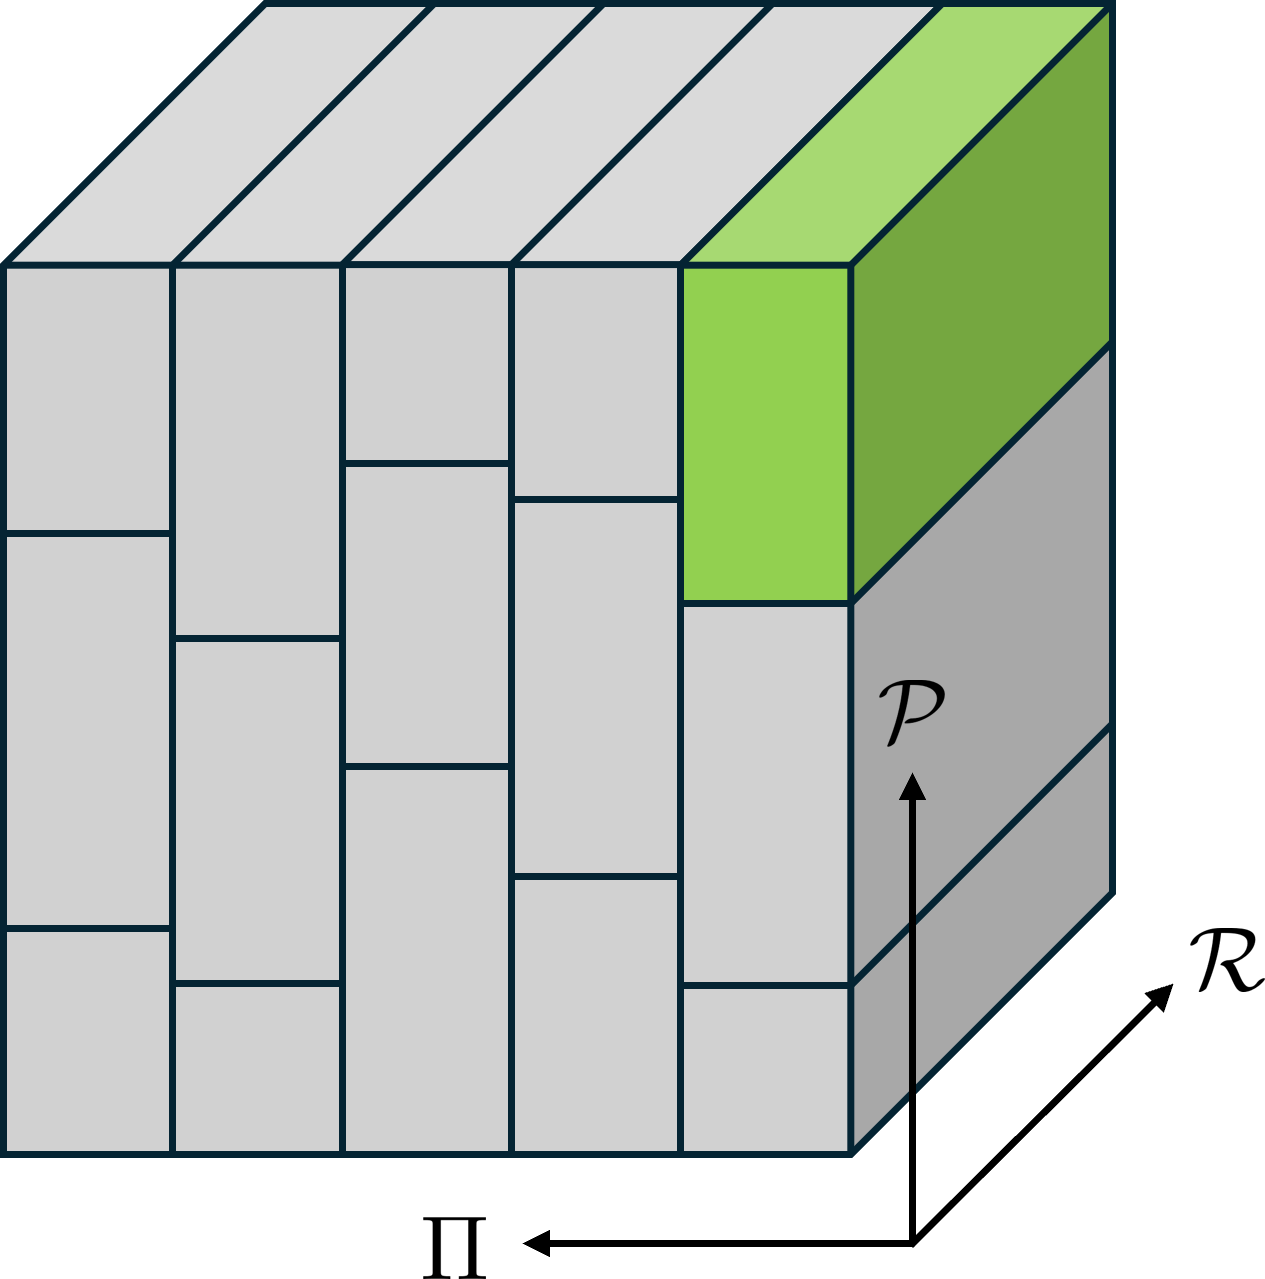
\includegraphics[width=0.3\textwidth]{Picture1.png}
\caption{Partitioning for hybrid MDPs}\label{fig: illustrate}
\end{figure}

\pref{fig: illustrate} illustrates the partition scheme over $\calM\times \Pi=\calP\times \calR\times \Pi$ described in \pref{assum: function approximation hybrid}. Each infoset $\phi$ (represented by the green block in \pref{fig: illustrate}) is associated with single policy $\pi_\phi$, a subset of transitions, and all reward functions. %Under a fixed policy $\pi$, transition $P$ and transition $P'$ should lie in the same $\phi$ if $Q^{\pi}(s,a; (P, R)) = Q^{\pi}(s,a; (P', R))$ for all $s,a,R$. 
As shown in \pref{fig: illustrate}, the partition over the $\calP$ space could be different for different $\pi$. 


\subsection{Algorithm and regret decomposition}
%\begin{align*}
%    \hair_\eta^{\Phi, D, \hattP_\Phi}(p, \nu; \rho) &=\E_{\pi\sim p} \E_{(\phi, P, R)\sim \nu}\E_{o\sim M_{P,R}(\cdot|\pi)} \\
%    &\qquad \left[V_{\hattP_\phi, R}(\pi_\phi) - V_{P,R}(\pi) - \frac{1}{\eta}\KL\left(\nu_{\bo{\phi}}(\cdot|\pi, o), \rho\right) - \right]
%\end{align*}
\begin{algorithm}[H]
    \caption{Model-free learning for the hybrid setting with bandit feedback and bilinear structure}
    \label{alg:MFHB}
    \jz{We don't need any specific algorithms anymmore, correct?}
    %\textbf{Input:} %Partition set $\Phi =  \left\{\phi_{\pi, f}: \pi \in \Pi, f \in \calF^\pi\right\}$,  $\rho_1(\phi) = \frac{1}{|\Phi|},\, \forall \phi \in \Phi$, 
   %epoch length $\tau$, and learning rate $\eta, \beta, \gamma$. \\
   Let $\rho_1(\phi) = \frac{1}{|\Phi|}$ for all $\phi$. \\
   \For{\textup{\textbf{epoch}} $k=1, 2, \ldots, \frac{T}{\tau}$}{
      %Given $ D^\pi_{\hbi}(\phi, \hattP_\phi||P)$ defined in \pref{eq:h-bi-div} and $D^\pi(\nu\|\rho)$ in \pref{eq: our divergence}, 
      Let $p_{k}, \nu_k$ be the solution of the minimax optimization: 
        \begin{align*}
            &\min_{p \in \Delta(\Pi)}\max_{\nu \in \Delta(\Psi)} \air_\eta^{\Phi, D}(p, \nu; \rho_t).    %\E_{\pi \sim p}\E_{(M,\pi^\star) \sim \nu}\left[V_{M}(\pi^\star) -V_{M}(\pi) - \frac{1}{\eta}\E_{o \sim M(\pi)}\left[\KL\left(\nu_{\bo{\phi}}(\cdot|\pi, o), \rho_k\right)\right] - \frac{1}{\eta}\E_{\phi \sim \rho_k}\left[ D^\pi_{\hbi}(\phi||M)\right]\right].
            \numberthis \label{eq:minmax hybrid}
        \end{align*}
         Sample $\pi_k  \sim p_k$. \\
         \For{$i=1,\ldots, \tau$}{
        Execute $\pi_k$ and observes $o_{k,h}^i = (s_{k,h}^i, a_{k,h}^i, r_{k,h}^i, s_{k,h+1}^i)$ for all $h$.
         }        
         Define
        \begin{align}
        &L_k(\phi) = \max\limits_{R\in\calR}\sum_{h=1}^H \left(\frac{1}{\tau} \sum_{i \in [\tau]}\ellest_h(\phi, R; o_{k,h}^i)\right)^2,\label{eq:adv_Lk}
             \\&\rho_{k+1} = \argmin_{\rho\in \Delta(\Phi)}\left\{\inner{\rho, L_k} + \frac{1}{\beta \tau}\sum_{i=1}^\tau \KL(\rho, (\nu_k)_{\bo{\phi}}(\cdot|\pi_k, o_k^i)) + \frac{1}{\gamma}\KL(\rho, \rho_k) \right\}. \label{eq:rho-hybrid 2}
        \end{align}
        % where $o_k=(o^i_{k,h})_{h\in[H],i\in[\tau]}$ is all observations in epoch $k$. 
    %      Solve $\nu_k$ as 
    %      \begin{align*}
    %         \nu_k =  \E_{\pi\sim p_k} \E_{(M,\pi^\star)\sim \nu} \left[
    % V_{M}(\pi^\star) - V_{M}(\pi) - \frac{2}{\eta}\E_{o \sim M(\pi)}\left[\KL(\nu_{\phi|\pi, o}, \, \rho_k)\right]- \frac{1}{\eta} \E_{\phi \sim \rho_k}\left[L^\pi(\phi, P, R)\right] \right].
    %      \end{align*}
    %      Define $o_k = (o_k^1,\cdots, o_k^{\tau})$, and set 
    %     \begin{align*}
    %         \rho_{k+1}(\phi) = \nu_k(\phi|\pi_k, o_k)\exp\left(-L_k(\phi)\right) \quad \text{and} \quad L_k(\phi) = \max_{R}\sum_{h=1}^H \left(\frac{1}{\tau} \sum_{i \in [\tau]}\ellest_h(\phi, w_{k,h}^i, R)\right)^2
    %     \end{align*}
    }
\end{algorithm}

The choices of diverges in \pref{alg:MFHB}: 
\begin{align}
    &D^\pi(\nu\|\rho) = \E_{\phi\sim \rho}\E_{(P,R) \sim \nu}\E_{o \sim M_{P,R}(\cdot|\pi)}\left[\KL\left(\nu_{\bo{\phi}}(\cdot|\pi, o), \rho\right) + \E_{P_\phi\sim z(\cdot|\phi)}\left[\tilD^\pi(\phi\|P) \right]\right]  ,  \label{eq:adv_div}
    \\& \tilD^\pi(\phi\|P) = \tilD_{\hbi}^\pi(\phi\|P) = \max_{R}\sum_{h=1}^H\left(\E^{\pi, P}\left[\ellest_h\l(\phi, R; o_h)\right]\right)^2  \label{eq:adv_bi_div}
\end{align}
%with the definition of $\Phi$ following \pref{assum: function approximation hybrid}. For a fixed comparator policy $\pi^\star$, let $\phi^\star$ be the aggregation such that  $\pi_{\phi^\star} = \pi^\star$ and for any $((P,R), \pi^\star) \in \phi$, we have $Q^{\pi^\star}(s,a, (P, R')) = Q^{\pi^\star}(s,a, (P^\star, R'))$ for any $s,a, R'$. 
Note that although we defined $L_k(\phi)$ in \pref{eq:adv_Lk} with the full observations $o_{k,h}^i$, only the observations of transition is really used in $L_k(\phi)$ while the reward observation is discarded. This is because we would like $L_k(\phi)$ to capture only the value error due to the transition error \emph{under the worst choice of the reward function}. This is also why the definition of $L_k(\phi)$ involves a maximization over $R$. % Instead, to tackle the adversarial rewards, we take a $\max_{R}$ to consider the worst case reward in $L_k(\phi)$. 
%Correspondingly, we only use the transition information in $o_h$ in \pref{eq:adv_bi_div}, and the expectation $\E^{\pi, P}$ is only related to transitions. 

The regret is decomposed as the following. With abuse of notation, we use $\pi_t, \rho_t, \nu_t$ to denote $\pi_k, \rho_k, \nu_k$ if $t$ is in epoch $k$. 
\iffalse
\begin{align*}
    &V_{P^\star, R_t}(\pi_{\phi^\star}) - \E_{\pi\sim p_t} [V_{P^\star, R_t}(\pi)]\\
    &= \E_{\pi\sim p_t}\left[ V_{\hatP_{\phi^\star}, R_t}(\pi_{\phi^\star}) - V_{P^\star, R_t}(\pi) - \frac{1}{\eta} D^{\pi}(\delta_{P^\star, R_t} \| \rho_t; \hatP_\Phi) \right]  + \frac{1}{\eta}  \E_{\pi\sim p_t} \left[D^\pi(\delta_{P^\star, R_t} \| \rho_t; \hatP_\Phi)\right] \\
    &\qquad \qquad + \left( V_{P^\star, R_t}(\pi_{\phi^\star}) - V_{\hatP_{\phi^\star}, R_t}(\pi_{\phi^\star})\right)   \\
    &\leq \max_{z} \E_{\pi\sim p_t}\left[ \E_{P_{\phi^\star}\sim z(\cdot|\phi^\star) } \left[V_{P_{\phi^\star}, R_t}(\pi_{\phi^\star})\right] - V_{P^\star, R_t}(\pi) - \frac{1}{\eta} D^{\pi}(\delta_{P^\star, R_t} \| \rho_t; z) \right]   + \frac{1}{\eta}   \E_{\pi\sim p_t} \left[D^\pi(\delta_{P^\star, R_t} \| \rho_t; \hatP_\Phi)\right] \\
    &\leq \max_\nu \max_{z} \E_{\pi\sim p_t}\E_{(\phi, P, R)\sim \nu}\left[ \E_{P_\phi\sim z(\cdot|\phi)} \left[V_{P_{\phi}, R}(\pi_{\phi})\right] - V_{P, R}(\pi) - \frac{1}{\eta} D^{\pi}(\nu \| \rho_t; z) \right]  \\
    &\qquad \qquad - \E_{\pi\sim p_t} \left[\breg_{D^{\pi}}\right] \\
    &\qquad \qquad + \frac{1}{\eta} \sum_{t=1}^T  \E_{\pi\sim p_t} \left[D^\pi(\delta_{P^\star, R_t} \| \rho_t; \hatP_\Phi)\right] \\
    %&\qquad \qquad + \underbrace{\frac{1}{\eta} \sum_h \E_{\phi\sim \rho} \left(\E^{\pi_t, P^\star}[\ellest_h(\phi, P_{\phi, t}, R_t; o_h)]\right)^2}_{\text{handle this separately}}
\end{align*}
\fi

\begin{align}
&\Reg(\pi_{\phi^\star}) \nonumber
%\\&= \E[\Reg(\pi^\star)] \nonumber
    \\&=\sum_{t=1}^T \left(V_{M_t}(\pi_{\phi^\star}) - \E_{\pi\sim p_t}[V_{M_t}(\pi)]\right)  \nonumber
    \\&\le   \sum_{t=1}^T \underbrace{\min_{p \in \Delta(\Pi)}\max_{\nu \in \Delta(\calM \times \Pi)}\air^{\Phi, D}_\eta(p,\nu; \rho_t)}_{\textbf{Complexity}} + \frac{1}{\eta} \underbrace{\sum_{t=1}^T \E_{\pi\sim p_t}\left[D^{\pi}(\delta_{M_t,\pi^\star}\|\rho_t) - \breg_{D^{\pi}(\cdot\|\rho_t)}(\delta_{M_t,\pi^\star}, \nu_t)\right] }_{\est}. \label{eq:adv_bi_init_decom 2}
\end{align}




% $\left(X(\phi')^\top\E_{R \sim \nu(\cdot|\phi)}\left[\theta(R)\right] - X(\phi')^\top\E_{R \sim \nu}\left[\theta(R)\right]\right)$

% \subsection{Bounding the estimation error}


% Since every $M_t = (P^\star, R_t)$ shares the same transition $P^\star$, every $(M_t, \pi^\star)$ lies in $\phi^\star$. From the definition of divergence in \pref{eq:adv_div} and \pref{eq:adv_bi_div},  as we divide the $T$ rounds into $K$ epoch, we have
% \begin{align}
%     &\est\nonumber
%     \\&=   \sum_{t=1}^T \left(D^{\pi_t}(\delta_{M_t,\pi^\star}\|\rho_t) - \breg_{D^{\pi_t}(\cdot\|\rho_t)}(\delta_{M_t,\pi^\star}, \nu_t)\right) \nonumber
%     \\&=  \sum_{t=1}^T \Bigg(\log\left(\frac{1}{\rho_t(\phi^\star)}\right) +  \E_{\pi \sim p_t}\E_{\phi\sim \rho_t}\left[\sum_{h=1}^H\left(\E^{\pi, P^\star}\left[\ellest_h(\phi; o_h, R_t)\right]\right)^2  \right] \nonumber \\
%     &\qquad \qquad \qquad \qquad - \E_{\pi \sim p_t}\E_{o \sim M_t(\cdot|\pi)}\left[\KL\left(\delta_{\phi^\star}, (\nu_t)_{\bo{\phi}}(\cdot|\pi, o)\right) \right]\Bigg)\nonumber
%     \\&= \sum_{t=1}^T \E_{\pi \sim p_t}\E_{o \sim M_t(\cdot|\pi)}\left[\log\left(\frac{\nu_t(\phi^\star|\pi, o)}{\rho_t(\phi^\star)}\right)\right] +  \sum_{t=1}^T\E_{\pi \sim p_t}\E_{\phi\sim \rho_t}\left[D_{\bi}^{\pi}(\phi||P^\star, R_t)\right] \nonumber
%     \\&\le \sum_{k=1}^K \E_{\pi \sim p_k}\left[\sum_{i=1}^\tau \E_{o \sim M_{(k-1)\tau + i}(\cdot|\pi)}\left[\log\left(\frac{\nu_k(\phi^\star|\pi, o)}{\rho_k(\phi^\star)}\right)\right]\right] \nonumber \\
%     &\qquad \qquad \qquad \qquad + \sum_{k=1}^K\sum_{i=1}^{2\tau}\E_{\pi \sim p_k}\E_{\phi\sim \rho_k}\left[\max_{R \in \mathcal{R}}D_{\bi}^{\pi}(\phi||P^\star, R)\right]\label{eq:est_adv_fir 2}
% \end{align}
% % With sum of KL in the update of $\rho_{k+1}$, we have a term
% % \begin{align*}
% %     \frac{1}{\eta} \sum_{k=1}^K\sum_{i=1}^\tau\log\left(\frac{\rho_{k}(\phi^\star)}{\nu_k(\phi^\star|\pi_k,o_k^i)}\right) 
% % \end{align*}
% where the second equality uses the fact that
% \begin{align*}
%     \breg_{D^{\pi}(\cdot\|\rho_t)}(\nu, \nu') = \E_{M \sim \nu}\E_{o \sim M(\cdot|\pi)}\left[\KL\left(\nu_{\bo{\phi}}(\cdot|\pi, o), \nu_{\bo{\phi}}'(\cdot|\pi, o)\right)\right].
% \end{align*}

% Applying \pref{lem: online esitmation epoch general} with
% \begin{align*}
%     \ellest_h(\phi, R; o^i_{k,h}) &= f_{\phi}(s^i_{k,h}, a^i_{k,h}; R) - R(s^i_{k,h}, a^i_{k,h}) - f_\phi(s^i_{k,h+1}; R) \\
%     \ell^j_{k,h}(\phi) &= \ellest_h(\phi, R^j; o^i_{k,h}), \qquad \text{where} \ \ R^j(s,a) = \varphi(s,a)^\top \mathbf{e}_j \\
%     F_k^i(\rho) &= \KL(\rho, (\nu_k)_{\bo{\phi}} (\cdot|\pi_k, o^i_k) )
% \end{align*}
% % \jz{ Do we still need to bound the estimation error separately here?}
% % \jz{I mean using the theorem 7}
% % \HL{I think we can directly use the lemma 33 you wrote for $\sum_{k=1}^K\sum_{i=1}^{2\tau}\E_{\pi \sim p_k}\E_{\phi\sim \rho_k}\left[\max_{R \in \mathcal{R}}D_{\bi}^{\pi}(\phi||P^\star, R)\right]$, then}
% % \HL{It seems we can use theorem 7 everywhere? Actually where is the proof for theorem 7. For hybrid bilinear $N = d$?}
% % \jz{Theorem 7 is for non bc and theorem 8 for bc}\jz{Yes. the proof is in appendix H}
% % \HL{Cool I will delete the redundant proof}

% We have
% \begin{align*}
%         % &\sum_{k=1}^K\sum_{i=1}^{2\tau}\E_{\phi \sim \rho_k}\left[\left(\E^{P^\star, \pi_k}\left[\ell_h(\phi;o_{k,h}^i)\right]\right)^2\right] 
%         &\sum_{k=1}^K\sum_{i=1}^{2\tau}\E_{\pi \sim p_k}\E_{\phi\sim \rho_k}\left[\max_{R \in \mathcal{R}}D_{\bi}^{\pi}(\phi||P^\star, R)\right]
%         \\ &\le \frac{\log|\Phi|}{\gamma} +  \sum_{k=1}^K \left(\sum_{i=1}^{2\tau}(  F_k^i(\delta_{\phi^\star}) - F_k^i(\rho_{k+1}) - \breg_{F_k^i}(\delta_{\phi^\star}, \rho_{k+1}) \right) + 90B^2HT^{\frac{1}{3}}N^\frac{2}{3}
%         \\&=  \sum_{k=1}^K \sum_{i=1}^{2\tau} \log\left(\frac{\rho_{k+1}(\phi^\star)}{\nu_k(\phi^\star|\pi_k,o_k^i)}\right) - \sum_{k=1}^K\sum_{i=1}^{2\tau}\KL(\rho_{k+1}, (\nu_k)_{\bo{\phi}} (\cdot|\pi_k, o^i_k) ) + 90B^2HT^{\frac{1}{3}}N^\frac{2}{3}
%         \\&\le  \sum_{k=1}^K \sum_{i=1}^{2\tau} \log\left(\frac{\rho_{k}(\phi^\star)}{\nu_k(\phi^\star|\pi_k,o_k^i)}\right) + \sum_{k=1}^K \sum_{i=1}^{2\tau} \log\left(\frac{\rho_{k+1}(\phi^\star)}{\rho_k(\phi^\star)}\right) + 90B^2HT^{\frac{1}{3}}\log|\Phi|N^\frac{2}{3} +  \frac{\log|\Phi|}{\gamma}
% \end{align*}
% Thus, we have
% \begin{align*}
%     &\E\left[\est\right]
%     \\&\le \sum_{k=1}^K \E_{\pi \sim p_k}\left[\sum_{i=1}^\tau \E_{o \sim M_{(k-1)\tau + i}(\cdot|\pi)}\left[\log\left(\frac{\nu_k(\phi^\star|\pi, o)}{\rho_k(\phi^\star)}\right)\right]\right] \nonumber \\
%     &\qquad \qquad \qquad \qquad + \sum_{k=1}^K\sum_{i=1}^{2\tau}\E_{\pi \sim p_k}\E_{\phi\sim \rho_k}\left[\max_{R \in \mathcal{R}}D_{\bi}^{\pi}(\phi||P^\star, R)\right]
% \end{align*}



% Old bound
% \begin{align*}
%     &\frac{1}{8}\sum_{k=1}^K\E_{\pi \sim p_k}\E_{\phi \sim \rho_k}\left[\max_{R \in \calR} D_{\hbi}^{\pi}(\phi\|P^\star, R)\right] 
%     \\&\le  \frac{1}{\beta}\sum_{k=1}^K\sum_{i=1}^\tau\log\left(\frac{\rho_{k+1}(\phi^\star)}{\nu_k(\phi^\star|\pi_k,o_k^i)}\right) + \frac{1}{\gamma}\sum_{k=1}^K\log\left(\frac{\rho_{k+1}(\phi^\star)}{\rho_k(\phi^\star)}\right) + 3HK\epsilon_{\conc}^2 + 4HL^2\log(|\Phi|/\delta)
%     \\&\leq \frac{1}{\beta}\sum_{k=1}^K\sum_{i=1}^\tau\log\left(\frac{\rho_{k}(\phi^\star)}{\nu_k(\phi^\star|\pi_k,o_k^i)}\right) + \left(\frac{1}{\gamma} + \frac{\tau}{\beta}\right)\log|\Phi| + \frac{6HK\log\left(KH|\Phi||\calR|/\delta\right)}{\tau}+ 4HL^2\log(|\Phi|/\delta). 
% \end{align*}





% \cw{Remove the rest of the proof for $\est$ and use the result in \pref{app: batching improve} with 
% \begin{align*}
%     \ellest_h(\phi, R; o^i_{k,h}) &= f_{\phi}(s^i_{k,h}, a^i_{k,h}; R) - R(s^i_{k,h}, a^i_{k,h}) - f_\phi(s^i_{k,h+1}; R) \\
%     \ell^j_{k,h}(\phi) &= \ellest_h(\phi, R^j; o^i_{k,h}), \qquad \text{where} \ \ R^j(s,a) = \varphi(s,a)^\top \mathbf{e}_j \\
%     F_k^i(\rho) &= \KL(\rho, (\nu_k)_{\bo{\phi}} (\cdot|\pi_k, o^i_k) )
% \end{align*}


% }

% Now we show that the estimation error can be well-bounded. Recall the update rule of $\rho_{k+1}$ (\pref{eq:rho-hybrid 2}): 
% \begin{align*}
%     \rho_{k+1} = \argmin_{\rho\in \Delta(\Phi)}\left\{ 
% \inner{\rho, L_k} + \frac{1}{\beta}\sum_{i=1}^\tau\KL(\rho, (\nu_k)_{\bo{\phi}}(\cdot|\pi_k, o_k^i) + \frac{1}{\gamma}\KL(\rho, \rho_k) \right\}. 
% \end{align*}
% where $L_k(\phi) =\max_R \sum_{h=1}^H\big(\frac{1}{\tau}\sum_{i=1}^{\tau} \ellest_h(\phi; o_{k,h}^i, R)\big)^2$. From \pref{lem: bregman}, we have
% \begin{align*}
%     &\inner{\rho_{k+1}, L_k} + \frac{1}{\beta}\sum_{i=1}^\tau\KL(\rho_{k+1}, (\nu_k)_{\bo{\phi}}(\cdot|\pi_k, o_k^i)) + \frac{1}{\gamma} \KL(\rho_{k+1}, \rho_k)
%     \\&\le \inner{\delta_{\phi^\star}, L_k} + \frac{1}{\beta}\sum_{i=1}^\tau\KL(\delta_{\phi^\star}, (\nu_k)_{\bo{\phi}}(\cdot|\pi_k, o_k^i)) + \frac{1}{\gamma} \KL(\delta_{\phi^\star}, \rho_k) \\
%     &\qquad \qquad \qquad \qquad -  \frac{1}{\beta}\sum_{i=1}^\tau\KL\left(\delta_{\phi^\star}, \rho_{k+1} \right) - \frac{1}{\gamma} \KL\left(\delta_{\phi^\star}, \rho_{k+1} \right)
% \end{align*}
% Thus, by setting $\gamma = \frac{1}{2HL^2}$, we have $0 \le \gamma L_k \le \frac{1}{2}$ and
% \begin{align*}
%     &\inner{\rho_{k}, L_k} 
%     \\&\le \inner{\rho_k - \rho_{k+1}, L_k} -  \frac{1}{\gamma}\KL(\rho_{k+1}, \rho_k) + L_k(\phi^\star) + \frac{1}{\beta}\sum_{i=1}^\tau\log\left(\frac{\rho_{k+1}(\phi^\star)}{\nu_k(\phi^\star|\pi_k,o_k^i)}\right) + \frac{1}{\gamma}\log\left(\frac{\rho_{k+1}(\phi^\star)}{\rho_k(\phi^\star)}\right) 
%     \\&\le \gamma \inner{\rho_k, L_k^2} + L_k(\phi^\star) + \frac{1}{\beta}\sum_{i=1}^\tau\log\left(\frac{\rho_{k+1}(\phi^\star)}{\nu_k(\phi^\star|\pi_k,o_k^i)}\right) + \frac{1}{\gamma}\log\left(\frac{\rho_{k+1}(\phi^\star)}{\rho_k(\phi^\star)}\right) \tag{\pref{lem:stability}}
%     \\&\le \frac{1}{2}\cdot\inner{\rho_k, L_k} + L_k(\phi^\star) + \frac{1}{\beta}\sum_{i=1}^\tau\log\left(\frac{\rho_{k+1}(\phi^\star)}{\nu_k(\phi^\star|\pi_k,o_k^i)}\right) + \frac{1}{\gamma}\log\left(\frac{\rho_{k+1}(\phi^\star)}{\rho_k(\phi^\star)}\right). 
% \end{align*}
% This implies
% \begin{align}
%     \frac{1}{2}\E_{\phi \sim \rho_k}\left[L_k(\phi)\right] \le L_k(\phi^\star) + \frac{1}{\beta}\sum_{i=1}^\tau\log\left(\frac{\rho_{k+1}(\phi^\star)}{\nu_k(\phi^\star|\pi_k,o_k^i)}\right) + \frac{1}{\gamma}\log\left(\frac{\rho_{k+1}(\phi^\star)}{\rho_k(\phi^\star)}\right)  \label{eq:rho_no_conc_adv}
% \end{align}
% By Hoeffding's inequality and union bound, with probability at least $1-\delta$, for any $k\in[K]$, $h\in[H]$, and any $\phi \in \Phi, R \in \calR$, we have
% \begin{align*}
% \left|\frac{1}{\tau} \sum_{i \in [\tau]}\ellest_h(\phi; o_{k,h}^i, R) -  \E^{ \pi_k,\, P^\star}\left[\ellest_h(\phi; o_h, R)\right]\right| \le \sqrt{\frac{2\log\left(KH|\Phi||\calR|/\delta\right)}{\tau}} = \epsilon_{\conc}. 
% \end{align*}
% Recall $D_{\hbi}^\pi(\phi\|P^\star, R) = \sum_{h=1}^H  \left(\E^{\pi, P^\star}\left[\ellest_h(\phi, o_h, R)\right]\right)^2$. The concentration inequality together with the inequality $(u+v)^2\leq 2u^2 + 2v^2$ imply for every $\phi\in\Phi$ and $R\in\calR$ and $k\in[K]$,%and define $L_k(\phi, R) = \sum_{h=1}^H \left(\frac{1}{\tau} \sum_{i \in [\tau]}\ellest_h(\phi, o_{k,h}^i, R)\right)^2$, we have 
% \begin{align*}
%     &\sum_{h=1}^H \left(\frac{1}{\tau} \sum_{i \in [\tau]}\ellest_h(\phi, o_{k,h}^i, R)\right)^2 \le 2 D_{\hbi}^{\pi_k}(\phi\|P^\star, R)  + 2H\epsilon_{\conc}^2,
%      \\&\sum_{h=1}^H \left(\frac{1}{\tau} \sum_{i \in [\tau]}\ellest_h(\phi, o_{k,h}^i, R)\right)^2 \ge \frac{1}{2}D_{\hbi}^{\pi_k}(\phi\|P^\star, R)  -H\epsilon_{\conc}^2. 
% \end{align*}
% % From Lemma A.3 in \cite{foster2021statistical}, with probability at least $1-\delta$, for any $\phi \in \Phi$, we have
% % \begin{align*}
% %    \frac{1}{2}\sum_{k=1}^K \E_{\pi \sim p_k}\left[L^\pi(\phi, P^\star, R)\right] \le   \sum_{k=1}^K D_{bi}^{\pi_k}(\phi||P^\star, R_k) + 4H\log(|\Phi|/\delta). 
% % \end{align*}
% These imply 
% \begin{align}
%     L_k(\phi)&=\max_{R\in\calR}\sum_{h=1}^H \left(\frac{1}{\tau} \sum_{i \in [\tau]}\ellest_h(\phi, o_{k,h}^i, R)\right)^2 \le 2 \max_{R\in\calR} D_{\hbi}^{\pi_k}(\phi\|P^\star, R)  + 2H\epsilon_{\conc}^2,\label{eq:adv_conc1}
%      \\L_k(\phi)&=\max_{R\in\calR}\sum_{h=1}^H \left(\frac{1}{\tau} \sum_{i \in [\tau]}\ellest_h(\phi, o_{k,h}^i, R)\right)^2 \ge \frac{1}{2}\max_{R\in\calR} D_{\hbi}^{\pi_k}(\phi\|P^\star, R)  -H\epsilon_{\conc}^2. \label{eq:adv_conc2}
% \end{align}


% %Thus, let $R_0 =  \argmax_{R \in \calR} L_k(\phi, R)$ and $R_1 = \argmax_{R \in \calR} D_{\hbi}^{\pi_k}(\phi\|P^\star, R)$, for any $\phi \in \Phi$, since $L_k(\phi) = L_k(\phi, R_0)$, we have
% %\begin{align}
% %&L_k(\phi) - 2\max_{R \in \calR} D_{\hbi}^{\pi_k}(\phi\|P^\star, R) = L_k(\phi, R_0) - 2D_{\hbi}^{\pi_k}(\phi\|P^\star, R_0) + \underbrace{2D_{\hbi}^{\pi_k}(\phi\|P^\star, R_0) - 2D_{\hbi}^{\pi_k}(\phi\|P^\star, R_1)}_{\le 0} \le 2H\epsilon_{conc}^2 \label{eq:adv_conc1}
% %\\&\frac{1}{2}\max_{R \in \calR} D_{\hbi}^{\pi_k}(\phi\|P^\star, R) - L_k(\phi) = \frac{1}{2}D_{\hbi}^{\pi_k}(\phi\|P^\star, R_1) - L_k(\phi, R_1) + \underbrace{L_k(\phi, R_1) - L_k(\phi, R_0)}_{\le 0} \le H\epsilon_{conc}^2 \label{eq:adv_conc2}
% %\end{align}
% From Lemma A.3 in \cite{foster2021statistical}, with probability at least $1-\delta$, for any $\phi \in \Phi$, we have
% \begin{align}
%    \frac{1}{2}\sum_{k=1}^K \E_{\pi \sim p_k}\left[\max_{R \in \calR} D_{\hbi}^{\pi}(\phi||P^\star, R)\right] \le   \sum_{k=1}^K \max_{R \in \calR} D_{\hbi}^{\pi_k}(\phi||P^\star, R) + 4HL^2\log(|\Phi|/\delta).  \label{eq:adv_policy_conc}
% \end{align}

% Combining \pref{eq:rho_no_conc_adv}, \pref{eq:adv_conc1}, \pref{eq:adv_conc2}, \pref{eq:adv_policy_conc}, using the fact that $D_{\hbi}^{\pi}(\phi^\star||P^\star, R) = 0$ for every $\pi$, and summing over $k$, we have
% with probability at least $1-2\delta$,  \begin{align*}
%     &\frac{1}{8}\sum_{k=1}^K\E_{\pi \sim p_k}\E_{\phi \sim \rho_k}\left[\max_{R \in \calR} D_{\hbi}^{\pi}(\phi\|P^\star, R)\right] 
%     \\&\le  \frac{1}{\beta}\sum_{k=1}^K\sum_{i=1}^\tau\log\left(\frac{\rho_{k+1}(\phi^\star)}{\nu_k(\phi^\star|\pi_k,o_k^i)}\right) + \frac{1}{\gamma}\sum_{k=1}^K\log\left(\frac{\rho_{k+1}(\phi^\star)}{\rho_k(\phi^\star)}\right) + 3HK\epsilon_{\conc}^2 + 4HL^2\log(|\Phi|/\delta)
%     \\&\leq \frac{1}{\beta}\sum_{k=1}^K\sum_{i=1}^\tau\log\left(\frac{\rho_{k}(\phi^\star)}{\nu_k(\phi^\star|\pi_k,o_k^i)}\right) + \left(\frac{1}{\gamma} + \frac{\tau}{\beta}\right)\log|\Phi| + \frac{6HK\log\left(KH|\Phi||\calR|/\delta\right)}{\tau}+ 4HL^2\log(|\Phi|/\delta). 
% \end{align*}
% Putting this back to \pref{eq:est_adv_fir 2} and choose $\beta = 8\tau$, we have
% \begin{align*}
%     &\est\nonumber
%     \\&\le  \sum_{k=1}^K \E_{\pi \sim p_k}\left[\sum_{i=1}^\tau \E_{o \sim M_{(k-1)\tau + i}(\cdot|\pi)}\left[\log\left(\frac{\nu_k(\phi^\star|\pi, o)}{\rho_k(\phi^\star)}\right)\right]\right] +  \tau \sum_{k=1}^K\E_{\pi \sim p_k}\E_{\phi\sim \rho_k}\left[\max_{R \in \mathcal{R}}D_{\bi}^{\pi}(\phi||P^\star, R)\right] 
%     \\&\le \sum_{k=1}^K \E_{\pi \sim p_k}\left[\sum_{i=1}^\tau \E_{o \sim M_{(k-1)\tau + i}(\cdot|\pi)}\left[\log\left(\frac{\nu_k(\phi^\star|\pi, o)}{\rho_k(\phi^\star)}\right)\right]\right] +  \sum_{k=1}^K\sum_{i=1}^\tau\log\left(\frac{\rho_{k}(\phi^\star)}{\nu_k(\phi^\star|\pi_k,o_k^i)}\right)
%     \\& \qquad \qquad + \otil\left( \frac{HT\log(|\Phi||\calR|/\delta)}{\tau } + \tau HL^2\log(|\Phi|/\delta)\right). 
% \end{align*}
% where $\otil$ here only omits $\log(HT)$.
% Thus, taking expectation and use $K = \frac{T}{\tau}$, we have
% \begin{align*}
%     \E\left[\est\right] \le  \otil\left( \frac{HT\log(|\Phi||\calR|)}{\tau } + \tau HL^2\log(|\Phi|)\right) = \otil\left( HL\log|\Phi|\sqrt{T\log|\calR|} \right) 
% \end{align*}
% where we choose the optimal $\tau=\frac{\sqrt{T\log|\calR|}}{L}$. 



% % Now we move to bound the \textbf{complexity} term in \pref{eq:stoc_bi_init_decom}. From \pref{lem:adv_complexity}, we have
% % \begin{align*}
% %     \textbf{complexity} &\le T\cdot\mfdec_\eta^{\tilD,\Phi}
% %     \\&\le T\cdot\odec_\eta^{\tilD,\Phi}  + \eta T
% % \end{align*} \HL{Need prove this for adv settings}
% % Given the definition of $\tilD$ in \pref{eq:stoc_bi_div}, from Lemma 20 in \cite{liu2025decision}. 
% % \begin{itemize}
% %     \item If for every $\phi \in \Phi$, $\esttt(\pi_{\phi}) = \pi_{\phi}$, then $\odec_\eta^{\tilD,\Phi}  \le \order(dH\eta)$.
% %     \item If there exists $\phi \in \Phi$ such that $\esttt(\pi_{\phi}) \neq \pi_{\phi}$, then $\odec_\eta^{\tilD,\Phi}  \le \order(H\sqrt{d\eta})$ if $\eta \le \frac{1}{dH^2}$.
% % \end{itemize}



\subsection{Proof of \pref{thm: bilinear-adv}}
From \pref{thm: avg est}, with $N = d$, we have
\begin{align*}
    \E\left[\est\right] \le HB^2d^{\frac{2}{3}}T^{\frac{1}{3}}\log\left(|\Phi|\right)
\end{align*}
Combine with the complexity bound in \pref{lem: digdec_adv < d hbi}, we have the following results:

Thus, if for every $\phi \in \Phi$, $\esttt(\pi_{\phi}) = \pi_{\phi}$, and $B \le 1$,  we can bound the regret as 
\begin{align*}
    \E[\Reg(\pi_{\phi^\star})] \leq \otil\left(\eta^{\frac{1}{3}}d^{\frac{1}{3}}H^{\frac{2}{3}}\cdot T + \frac{ Hd^{\frac{2}{3}}T^{\frac{1}{3}}\log\left(|\Phi|\right)}{\eta}\right)
\end{align*}
which is $\otil\left(H^{\frac{3}{4}}d^{\frac{5}{12}}T^{\frac{5}{6}}\log(|\Phi|)^{\frac{1}{4}}\right)$
by choosing $\eta = H^{\frac{1}{4}}d^{\frac{1}{4}}T^{-\frac{1}{2}}\log(|\Phi|)^{\frac{3}{4}}$. %, $\tau = \sqrt{T}$, we have regret $\otil\left(\sqrt{dH^2L^2\log(|\Phi||\calR|)}T^{\frac{3}{4}}\right)$.


% \begin{itemize}
%     \item If $\esttt(\pi_{\phi}) = \pi_{\phi}$ for all $\phi$, then $\alpha = 0$, and $\max_\nu \qcom^{\Phi, \tilD_\hbi}_\eta(\nu) \le \order\left(\eta^{\frac{1}{3}}d^{\frac{1}{3}}H^{\frac{2}{3}}\right)$
%     \item  If there exists a $\phi$ such that  $\esttt(\pi_\phi) \neq \pi_{\phi}$, then setting $\alpha = 3H\sqrt{\eta d}$, we have $\max_\nu \qcom^{\Phi, \tilD_\hbi}_\eta(\nu) \le \order\left(\eta^{\frac{1}{6}}d^{\frac{1}{6}}H^{\frac{1}{3}}\right)$. 
% \end{itemize}

Otherwise, if there exists a $\phi$ such that $\esttt(\pi_{\phi}) \neq \pi_{\phi}$, then $B \le |\calA|$ , the regret bound is 
\begin{align*}
    \E[\Reg(\pi_{\phi^\star})] \leq \otil\left(\eta^{\frac{1}{6}}d^{\frac{1}{6}}H^{\frac{1}{3}}\cdot T  + \frac{ H|\calA|^2d^{\frac{2}{3}}T^{\frac{1}{3}}\log\left(|\Phi|\right)}{\eta}\right)
\end{align*}
which is $\otil\left(H^{\frac{4}{7}}d^{\frac{5}{21}}T^{\frac{19}{21}}|\calA|^{\frac{2}{7}}\log|\Phi|^{\frac{1}{7}}\right)$ by choosing $\eta = H^{\frac{4}{7}}d^{\frac{3}{7}}T^{-\frac{4}{7}}|\calA|^{\frac{12}{7}}\log(|\Phi|)$. 

\fi